\documentclass[english,xcolor={rgb,dvipsnames,table,usenames}, presentation]{beamer}

\mode<beamer> {

\usepackage{pgfpages}
\usecolortheme{magpie}
\setbeamercolor{normal text}{fg=white}
\usebeamercolor[fg]{normal text}
\setbeameroption{show notes}
\setbeameroption{show notes on second screen=right}
\setbeamerfont{note page}{size=\footnotesize}


}


\mode<handout> {

\usecolortheme{beaver}
\setbeamercolor{normal text}{fg=black}
\usebeamercolor[fg]{normal text}
\renewcommand{\textcolor}[1]{}

}



\usepackage{colortbl}
\usepackage{cancel}
\usepackage{multirow}
\usepackage{graphicx}
\usepackage{booktabs}
\usepackage[utf8]{inputenc}
\usepackage[T1]{fontenc}
\usepackage{colortbl}
\usepackage{pgfplots}
\usepackage{array,multirow,makecell}
\usepackage{dsfont}
\usepackage{stmaryrd}
\usepackage{multicol}
\usepackage{changepage}
\usepackage{amsmath}
\usepackage{amssymb}
\usepackage{amsfonts}
\usepackage{bm}
\usepackage[export]{adjustbox}
\usepackage{slashbox}
\usepackage{xcolor}
\usepackage{pict2e}
\usepackage{pifont}
\usepackage{eurosym}
\usepackage{tikz}
\usepackage{ulem}
\usepackage[customcolors]{hf-tikz}
\usetikzlibrary{arrows,intersections,positioning,shapes.arrows,decorations.markings}
\usepackage{hyperref}
\usepackage{mdframed}
\usepackage{listings}
\usepackage{caption}
\usepackage{subcaption}
\usepackage[backend=biber,bibencoding=utf8]{biblatex}
\usepackage{animate}
\usepackage{listings}
\usepackage{appendixnumberbeamer}
\usetikzlibrary{calc}
\usetikzlibrary{hobby}
\makeatletter % from https://tex.stackexchange.com/a/283273/121799
% Here we define the comparison macro for pairs (a,b)
% We assume decimal numbers acceptable to \ifdim tests
\long\def\xintdothis #1#2\xintorthat #3{\fi #1}%
\let\xintorthat \@firstofone

\captionsetup[figure]{labelfont={color=orange}}

\long\def\@thirdoffour  #1#2#3#4{#3}%
\long\def\@fourthoffour #1#2#3#4{#4}%

\def\IfFirstPairIsGreaterTF #1#2{\@IfFirstPairIsGreaterTF #1,#2,}%

\def\@IfFirstPairIsGreaterTF #1,#2,#3,#4,{%
    \ifdim #1\p@=#3\p@
       \xintdothis{%
         \ifdim #2\p@>#4\p@\expandafter\@firstoftwo
         \else\expandafter\@secondoftwo\fi}\fi
    \ifdim #1\p@>#3\p@\expandafter\@thirdoffour
                      \else\expandafter\@fourthoffour\fi
    \xintorthat{}%
}%

% not needed for numerical inputs
% \catcode`! 3
% \catcode`? 3

% Here there is a very strange \romannumeral0\romannumeral0, this is
% due to some convoluted scheme to avoid double spaces or no spaces
% in between coordinate pairs. Trust me.
\def\QSpairs {\romannumeral0\romannumeral0\qspairs }%
% first we check if empty list
\def\qspairs   #1{\expandafter\qspairs@a\romannumeral-`0#1(!)(?)}%
\def\qspairs@a #1(#2{\ifx!#2\expandafter\qspairs@abort\else
                        \expandafter\qspairs@b\fi (#2}%
\edef\qspairs@abort #1(?){\space\space}%
%
% we check if empty of single and if not pick up the first as Pivot:
\def\qspairs@b #1(#2)#3(#4){\ifx?#4\xintdothis\qspairs@empty\fi
                   \ifx!#4\xintdothis\qspairs@single\fi
                   \xintorthat \qspairs@separate {}{}{#2}(#4)}%
\def\qspairs@empty  #1(?){ }%
\edef\qspairs@single #1#2#3#4(?){\space\space(#3)}%
\def\qspairs@separate #1#2#3#4(#5)%
{%
    \ifx!#5\expandafter\qspairs@separate@done\fi
    \IfFirstPairIsGreaterTF {#5}{#3}%
          \qspairs@separate@appendtogreater
          \qspairs@separate@appendtosmaller {#5}{#1}{#2}{#3}%
}%
%
\def\qspairs@separate@appendtogreater #1#2{\qspairs@separate {#2 (#1)}}%
\def\qspairs@separate@appendtosmaller #1#2#3{\qspairs@separate {#2}{#3 (#1)}}%
%
\def\qspairs@separate@done\IfFirstPairIsGreaterTF #1#2%
    \qspairs@separate@appendtogreater
    \qspairs@separate@appendtosmaller #3#4#5#6(?)%
{%
    \expandafter\qspairs@f\expandafter
    {\romannumeral0\qspairs@b #4(!)(?)}{\qspairs@b #5(!)(?)}{ (#2)}%
}%
%
\def\qspairs@f #1#2#3{#2#3#1}%
%
% \catcode`! 12
% \catcode`? 12

\makeatother
\makeatletter % from https://tex.stackexchange.com/a/412901/121799
\newcommand{\Distance}[3]{% % from https://tex.stackexchange.com/q/56353/121799
\tikz@scan@one@point\pgfutil@firstofone($#1-#2$)\relax  
\pgfmathsetmacro{#3}{veclen(\the\pgf@x,\the\pgf@y)/28.45274}
}
\makeatother 
\newcount\nbofwords
\makeatletter% from https://tex.stackexchange.com/a/12819/121799
\def\myutil@empty{}
\def\multiwords#1 #2\@nil{% 
 \def\NextArg{#2}%
 \advance\nbofwords by  1 %   
 \expandafter\edef\csname word\@alph\nbofwords\endcsname{#1}% 
 \ifx\myutil@empty\NextArg
     \let\next\@gobble
 \fi
 \next#2\@nil
}%    
\def\GetWords#1{%
   \let\next\multiwords 
   \nbofwords=0 %
   \expandafter\next#1 \@nil %
}% 
\makeatother

\long\def\First(#1,#2){#1}
\long\def\Second(#1,#2){#2}
\tikzset{declare
function={interpolator(\x,\xmin,\xmax,\rmin,\rmax)=(\rmin+\rmax)/2+((\rmin-\rmax)/2)*cos((\x-\xmin)*(180/(\xmax-\xmin)));}}
%\tikzset{declare function={PotatoeRadius(\x,\angleA,\angleB,\angleC,\angleD,\distanceA,\distanceB,\distanceC,\distanceD)=\distanceA+(\x-\angleA)*((\distanceB-\distanceA)/(\angleB-\angleA)+(\x-\angleB)*(((-1)*((\distanceB-\distanceA)/(\angleB-\angleA))+(\distanceC-\distanceB)/(\angleC-\angleB))/(\angleC-\angleA)+(((-1)*(((-1)*((\distanceB-\distanceA)/(\angleB-\angleA))+(\distanceC-\distanceB)/(\angleC-\angleB))/(\angleC-\angleA))+((-1)*((\distanceC-\distanceB)/(\angleC-\angleB))+(\distanceD-\distanceC)/(\angleD-\angleC))/(\angleD-\angleB))*(\x-\angleC))/(\angleD-\angleA)));}}
%(\angleC*(\angleC-\angleD)*\angleD*((\distanceA-\distanceB)*(\angleC-\x)*(\angleD-\x)*\x+pow(\angleA,3)*(-(\angleC*pow(\angleD,2)*\distanceB)+\angleD*(\distanceB-\distanceC)*(\angleD-\x)*\x+\angleC*(\distanceB-\distanceD)*pow(\x,2)+pow(\angleC,2)*(\angleD*\distanceB+(-\distanceB+\distanceD)*\x))+pow(\angleB,3)*(-(\angleA*pow(\angleD,2)*\distanceC)-\angleD*(\distanceA-\distanceC)*(\angleD-\x)*\x+\angleA*(\distanceC-\distanceD)*pow(\x,2)+pow(\angleC,2)*(-(\angleD*\distanceA)+\angleA*\distanceD+\distanceA*\x-\distanceD*\x)+pow(\angleA,2)*(\angleD*\distanceC-\distanceC*\x+\distanceD*\x)+\angleC*(pow(\angleD,2)*\distanceA-pow(\angleA,2)*\distanceD+(-\distanceA+\distanceD)*pow(\x,2)))+pow(\angleA,2)*(-(\angleD*(\distanceB-\distanceC)*(\angleD-\x)*\x*(\angleD+\x))-pow(\angleC,3)*(\angleD*\distanceB+(-\distanceB+\distanceD)*\x)+\angleC*(pow(\angleD,3)*\distanceB+(-\distanceB+\distanceD)*pow(\x,3)))+\angleA*(pow(\angleD,2)*(\distanceB-\distanceC)*(\angleD-\x)*pow(\x,2)+pow(\angleC,3)*(pow(\angleD,2)*\distanceB+(-\distanceB+\distanceD)*pow(\x,2))-pow(\angleC,2)*(pow(\angleD,3)*\distanceB+(-\distanceB+\distanceD)*pow(\x,3)))+pow(\angleB,2)*(\angleD*(\distanceA-\distanceC)*(\angleD-\x)*\x*(\angleD+\x)+pow(\angleC,3)*(\angleD*\distanceA-\angleA*\distanceD-\distanceA*\x+\distanceD*\x)-pow(\angleA,3)*(\angleD*\distanceC+(-\distanceC+\distanceD)*\x)+\angleC*(-(pow(\angleD,3)*\distanceA)+pow(\angleA,3)*\distanceD+(\distanceA-\distanceD)*pow(\x,3))+\angleA*(pow(\angleD,3)*\distanceC+(-\distanceC+\distanceD)*pow(\x,3)))+\angleB*(-(pow(\angleD,2)*(\distanceA-\distanceC)*(\angleD-\x)*pow(\x,2))+pow(\angleC,3)*(-(pow(\angleD,2)*\distanceA)+pow(\angleA,2)*\distanceD+(\distanceA-\distanceD)*pow(\x,2))+pow(\angleA,3)*(pow(\angleD,2)*\distanceC+(-\distanceC+\distanceD)*pow(\x,2))+pow(\angleC,2)*(pow(\angleD,3)*\distanceA-pow(\angleA,3)*\distanceD+(-\distanceA+\distanceD)*pow(\x,3))-pow(\angleA,2)*(pow(\angleD,3)*\distanceC+(-\distanceC+\distanceD)*pow(\x,3))))/((\angleA-\angleB)*(\angleA-\angleC)*(\angleB-\angleC)*(\angleA-\angleD)*(\angleB-\angleD)*(\angleC-\angleD)));}}
\newcommand{\DrawArcAngle}[6][]{% just for emergencies
\pgfmathanglebetweenpoints{\pgfpointanchor{#3}{center}}{\pgfpointanchor{#2}{center}}
\xdef\angleA{\pgfmathresult}
\pgfmathanglebetweenpoints{\pgfpointanchor{#3}{center}}{\pgfpointanchor{#4}{center}}
\xdef\angleB{\pgfmathresult}
\draw[#1] ($(#3)+(\angleA:#5)$) arc [start angle=\angleA,end angle=\angleB,radius=#5]
#6;
}
\newcommand{\DrawPotato}[5][]{
\coordinate (PotatoCenter) at (barycentric cs:#2=1,#3=1,#4=1,#5=1);
\pgfmathanglebetweenpoints{\pgfpointanchor{PotatoCenter}{center}}{\pgfpointanchor{#2}{center}}
\xdef\angleA{\pgfmathresult}
\pgfmathanglebetweenpoints{\pgfpointanchor{PotatoCenter}{center}}{\pgfpointanchor{#3}{center}}
\xdef\angleB{\pgfmathresult}
\pgfmathanglebetweenpoints{\pgfpointanchor{PotatoCenter}{center}}{\pgfpointanchor{#4}{center}}
\xdef\angleC{\pgfmathresult}
\pgfmathanglebetweenpoints{\pgfpointanchor{PotatoCenter}{center}}{\pgfpointanchor{#5}{center}}
\xdef\angleD{\pgfmathresult}

\Distance{(PotatoCenter)}{(#2)}{\distanceA}
\Distance{(PotatoCenter)}{(#3)}{\distanceB}
\Distance{(PotatoCenter)}{(#4)}{\distanceC}
\Distance{(PotatoCenter)}{(#5)}{\distanceD}
\xdef\coordList{(\angleA,\distanceA) (\angleB,\distanceB) (\angleC,\distanceC) (\angleD,\distanceD)}%
\typeout{\coordList}
\xdef\sortedList{\QSpairs{\coordList}}%
\GetWords{\sortedList}
\xdef\NewList{\worda,\wordb,\wordc,\wordd}%
\xdef\NewList{\expandafter\First\worda/\expandafter\Second\worda, 
\expandafter\First\wordb/\expandafter\Second\wordb,
\expandafter\First\wordc/\expandafter\Second\wordc,
\expandafter\First\wordd/\expandafter\Second\wordd}% this list is not used
\xdef\angleA{\expandafter\First\worda}%
\xdef\distanceA{\expandafter\Second\worda}%
\xdef\angleB{\expandafter\First\wordb}%
\xdef\distanceB{\expandafter\Second\wordb}%
\xdef\angleC{\expandafter\First\wordc}%
\xdef\distanceC{\expandafter\Second\wordc}%
\xdef\angleD{\expandafter\First\wordd}%
\xdef\distanceD{\expandafter\Second\wordd}%
\begin{scope}[shift=(PotatoCenter)]
\draw[#1,smooth,samples=50] plot[variable=\x,domain=\angleA:\angleB] %
(\x:{interpolator(\x,\angleA,\angleB,\distanceA,\distanceB)})
-- 
plot[variable=\x,domain=\angleB:\angleC] %
(\x:{interpolator(\x,\angleB,\angleC,\distanceB,\distanceC)})
--
plot[variable=\x,domain=\angleC:\angleD] %
(\x:{interpolator(\x,\angleC,\angleD,\distanceC,\distanceD)})
--
plot[variable=\x,domain=\angleD:{\angleA+360}] %
(\x:{interpolator(\x,\angleD,{\angleA+360},\distanceD,\distanceA)});
\end{scope}
}

\definecolor{links}{HTML}{2A1B81}
\hypersetup{colorlinks,linkcolor=,urlcolor=links}

\tikzset{style green/.style={
    set fill color=green!50!lime!60,
    set border color=white,
  },
  style cyan/.style={
    set fill color=cyan!90!blue!60,
    set border color=white,
  },
  style orange/.style={
    set fill color=orange!80!red!60,
    set border color=white,
  },
  hor/.style={
    above left offset={-0.15,0.31},
    below right offset={0.15,-0.125},
    #1
  },
  ver/.style={
    above left offset={-0.1,0.3},
    below right offset={0.15,-0.15},
    #1
  }
}

\newcommand{\tikzmark}[2][minimum width=6cm,minimum height=1.5cm]{
\tikz[remember picture, overlay]
\node[anchor=west,
inner sep=0pt,
outer sep=6pt,
xshift=-0.5em,
yshift=-3ex,
#1](#2){};
}

\newcommand{\norm}[1]{\left\lVert#1\right\rVert}

\addbibresource{biblio.bib}

\newcommand{\cmark}{\ding{51}}
\newcommand{\xmark}{\ding{55}}

\setcellgapes{1pt}
\makegapedcells
\newcolumntype{R}[1]{>{\raggedleft\arraybackslash }b{#1}}
\newcolumntype{L}[1]{>{\raggedright\arraybackslash }b{#1}}
\newcolumntype{C}[1]{>{\centering\arraybackslash }b{#1}}

\DeclareMathOperator*{\argmin}{\arg\!\min}
\DeclareMathOperator*{\argmax}{\arg\!\max}

\newcommand{\xuparrow}[1]{%
  {\left\uparrow\vbox to #1{}\right.\kern-\nulldelimiterspace}
}

\renewcommand*{\bibfont}{\small}

\tikzset{
  treenode/.style = {shape=rectangle, rounded corners,
                     draw, align=center,
                     top color=white, bottom color=blue!20},
  root/.style     = {treenode, font=\Huge, bottom color=red!30},
  env/.style      = {treenode, font=\ttfamily\Large},
  dummy/.style    = {circle,draw,color=black}
}

\newcommand\rstyle{%
  \NoAutoSpacing
  \lstset{%
    language=R,
    alsoletter={_},
otherkeywords={install_github},             % Add keywords here
%    basicstyle=\small,
    keywordstyle=\color{blue},
    stringstyle=\color{green},
%    numbers=left,
%    numberstyle=\tiny,
%    numbersep=5pt,
  numbers=left,                   % where to put the line-numbers
  numberstyle=\tiny\color{blue},  % the style that is used for the line-numbers
  stepnumber=1,                   % the step between two line-numbers. If it is 1, each line
                                  % will be numbered
  numbersep=5pt,                  % how far the line-numbers are from the code
  showspaces=false,               % show spaces adding particular underscores
  showstringspaces=false,         % underline spaces within strings
  showtabs=false,                 % show tabs within strings adding particular underscores
  breaklines=true,                % sets automatic line breaking
  breakatwhitespace=false,        % sets if automatic breaks should only happen at whitespace
    frame=single%
  }%
}

\lstnewenvironment{rlisting}
{\rstyle}{}

\newcommand\rinline[1]{{\rstyle\lstinline!#1!}}

% Allows the use of \toprule, \midrule and \bottomrule in tables

%----------------------------------------------------------------------------------------
%	TITLE PAGE
%----------------------------------------------------------------------------------------

\title[Soutenance]{Formalisation et étude de problématiques \\ de scoring en risque de crédit \\ {\vspace*{0.5cm} \small Inférence de rejet, discrétisation de variables et interactions, \\ arbres de régression logistique}}

\author{Soutenance de thèse d'Adrien Ehrhardt \\ {\footnotesize
Encadré par Christophe Biernacki, Philippe Heinrich, Vincent Vandewalle
}}

\institute[CACF - Inria]

\date{Villeneuve d'Ascq, 30/09/2019} % Date, can be changed to a custom date

\titlegraphic{%
    
\includegraphics[width=2.5cm]{figures/inria.png}~%
    
\includegraphics[width=4cm]{figures/logo.png}%
}

\AtBeginSection[]{
  \begin{frame}
  \vfill
  \centering
  \begin{beamercolorbox}[sep=8pt,center,shadow=true,rounded=true]{title}
    \usebeamerfont{title}\insertsectionhead\par%
  \end{beamercolorbox}
  \vfill
  \end{frame}
}

\tikzset{
    myarrow/.style={
        draw,
        fill=orange,
        single arrow,
        minimum height=3.5ex,
        single arrow head extend=1ex
    }
}

\tikzstyle{interrupt}=[
    postaction={
        decorate,
        decoration={markings,
                    mark= at position 0.5 
                          with
                          {
                            \fill[black] (-0.1,-0.3) rectangle (0.1,0.3);
                            \draw (-0.1,0.3) -- (-0.1,-0.3)
                                  (0.1,0.3) -- (0.1,-0.3);
                          }
                    }
                }
]

\newlength\mylinewidth
\setlength\mylinewidth{0.4pt}

\tikzset{
    ultra thin/.style= {line width=0.25\mylinewidth},
    very thin/.style=  {line width=0.5\mylinewidth},
    thin/.style=       {line width=\mylinewidth},
    semithick/.style=  {line width=1.5\mylinewidth},
    thick/.style=      {line width=2\mylinewidth},
    very thick/.style= {line width=3\mylinewidth},
    ultra thick/.style={line width=4\mylinewidth},
    every picture/.style={semithick}
}




\addtobeamertemplate{navigation symbols}{}{%
    \usebeamerfont{footline}%
    \usebeamercolor[fg]{footline}%
    \hspace{1em}%
    \insertframenumber/\inserttotalframenumber
}

\lstset{language=R}

\newcommand{\appropto}{\mathrel{\vcenter{
  \offinterlineskip\halign{\hfil$##$\cr
    \propto\cr\noalign{\kern2pt}\sim\cr\noalign{\kern-2pt}}}}}

\newcommand\q{{\bm{q}}}
\newcommand\s{q}
\newcommand\Q{\mathcal{Q}}
\newcommand\ag{\bm{\alpha}}
\newcommand{\bth}{\boldsymbol{\theta}} 
\newcommand{\bc}{\boldsymbol{c}} 
\newcommand{\bx}{\boldsymbol{x}} 
\newcommand{\tx}{\textbf{x}}
\newcommand{\bs}{\boldsymbol{s}} 
\newcommand{\ts}{\textbf{s}}
\newcommand{\be}{\boldsymbol{e}} 
\newcommand{\te}{\textbf{e}}
\newcommand{\by}{\boldsymbol{y}} 
\newcommand{\ty}{\textbf{y}}
\newcommand{\f}{\text{f}}
\newcommand{\nf}{\text{nf}}
\newcommand{\yslant}{0.5}
\newcommand{\xslant}{-0.6}
\newcommand{\tr}{T}
\newcommand{\bqk}{\bm{\mathfrak{q}}}

\def\mybar#1#2#3{%%
\begin{tabular}{@{}l@{}} {\scriptsize #1} \\ {\scriptsize #2} \\ {\scriptsize #3} \end{tabular} & \resizebox{.05#1\textwidth}{0.7cm}{\begin{tabular}{@{}l@{}}{\color{green}\rule[0pt]{#1bp}{10pt}} \\ {\color{orange}\rule[0pt]{#2bp}{10pt}} \\ {\color{red}\rule[0pt]{#3bp}{10pt}} \end{tabular}}}

\def\myobar#1#2#3{%%
\begin{tabular}{@{}l@{}} {\scriptsize #1} \\ {\scriptsize #2} \\ {\scriptsize #3} \end{tabular} & \resizebox{.05#2\textwidth}{0.7cm}{\begin{tabular}{@{}l@{}}{\color{orange}\rule[0pt]{#1bp}{10pt}} \\ {\color{green}\rule[0pt]{#2bp}{10pt}} \\ {\color{orange}\rule[0pt]{#3bp}{10pt}}\end{tabular}}}

\pgfmathdeclarefunction{gauss}{2}{\pgfmathparse{1/(#2*sqrt(2*pi))*exp(-((x-#1)^2)/(2*#2^2))}}

\newcommand{\myGlobalTransformation}[2]
{
    \pgftransformcm{1}{0}{0.4}{0.5}{\pgfpoint{#1cm}{#2cm}}
}


\newcommand{\myGlobalTransformationbis}[2]
{
    \pgftransformcm{1}{0}{0.4}{0.3}{\pgfpoint{#1cm}{#2cm}}
}

\newcommand{\gridThreeD}[3]
{
    \begin{scope}
        \myGlobalTransformation{#1}{#2};
        \draw [#3,step=7cm] grid (7,7);
    \end{scope}
}

\tikzstyle myBG=[line width=3pt,opacity=1.0]

\newcommand{\drawLinewithBG}[2]
{
    \draw[white,myBG]  (#1) -- (#2);
    \draw[black,very thick] (#1) -- (#2);
}

\newcommand{\graphLinesHorizontal}
{
    \drawLinewithBG{1,1}{7,1};
    \drawLinewithBG{1,3}{7,3};
    \drawLinewithBG{1,5}{7,5};
    \drawLinewithBG{1,7}{7,7};
}

\newcommand{\graphLinesVertical}
{
    %swaps x and y coordinate (hence vertical lines):
    \pgftransformcm{0}{1}{1}{0}{\pgfpoint{0cm}{0cm}}
    \graphLinesHorizontal;
}

\newcommand{\graphThreeDnodes}[2]
{
    \begin{scope}
        \myGlobalTransformation{#1}{#2};
        \foreach \x in {1,3,5,7} {
            \foreach \y in {1,3,5,7} {
                \node at (\x,\y) [circle,fill=black,scale=0.3] {};
                %this way circle of nodes will not be transformed
            }
        }
    \end{scope}
}

\begin{document}


\frame[plain]{\titlepage}

\note{Merci aux rapporteurs pour le temps consacré à la lecture du manuscrit, aux membres du jury pour leur disponibilité pour cette soutenance de thèse intitulée... 

\bigskip

On reviendra sur ce qu'on entend par scoring dans ce qui suit

\bigskip

Thèse encadrée par... préparée au sein de... et, s'agissant d'une CIFRE, chez CACF}





\begin{frame}

%%%%%%%%%%%%%%%%
\note{Je vais dans un premier temps introduire le contexte industriel et formalisation par l'introduction de notations. 

\medskip

Le premier apport de cette thèse, la Réintégration de refusés ou inférence de rejet.

\medskip

La sous-partie prépondérante de la thèse. Ce qu'on a mis dans le terme ``quantification'' à savoir la discrétisation de prédicteurs continus et le regroupement de modalités de variables catégorielles.

\medskip

Choix de passer sous silence les interactions.

\medskip

Dernière partie de thèse que l'on peut interpréter comme une segmentation prédictive : les arbres de régression logistique. Et quelques mots de conclusion.}
%%%%%%%%%%%%%%%%



\frametitle{Table of Contents}
\tableofcontents[hideallsubsections]
\end{frame}



\section{Context and notations}

\note{On se place dans la peau d'un chargé d'études statistiques qui a en face de lui un tel tableau.}

\subsection{industrial setting}

\begin{frame}<handout:0>
\frametitle{\secname: \subsecname}




%%%%%%%%%%%%%%%%%%%%
\note{Collecte des caractéristiques de demandeurs de crédit à la consommation.

\medskip

On connaît pour certains la performance de remboursement, c-à-d les clients financés.

\medskip

On cherche à estimer une probabilité de défaut de ces emprunteurs pour l'appliquer aux nouveaux demandeurs et décider de leur acceptation crédit.

\medskip

On passe traditionnellement par 6 étapes...

\medskip

On sélectionne les variables prédictives du remboursement.

\medskip

On effectue une régression logistique et une transformation qui donne le score.

\medskip

On se donne enfin un seuil en-dessous duquel les clients sont refusés.}
%%%%%%%%%%%%%%%%%%%%




\only<1-6>{
\begin{table}
\centering
\begin{tiny}
\hspace*{-0.7cm}\begin{tabular}{p{1.7cm}|p{1.1cm}|p{1cm}|p{1.4cm}|p{1.5cm}||p{0.6cm}|p{1cm}}
\textcolor <4,6> {green} {\textbf<4,6>{Job}} & \only<1-3>{Home} & \only<1-3>{Time in job} & \textcolor <4,6> {green} {\textbf<4,6>{Family status}} & \textcolor <4,5> {green} {\textbf<4,5>{Wages}} & \only<8->{\textcolor{green}{\textbf{Score}}} & Repayment \\
\hline
\textcolor <4,6> {green} {\textbf<4,6>{\only<1-5>{Craftsman} \only<6->{?+Low-qualified}}} & \only<1-3>{Owner} & \only<1-3>{20} & \textcolor <4,6> {green} {\textbf<4,6>{\only<1-5>{Widower}  \only<6>{?+Alone}}} & \textcolor <4-5> {green} {\textbf<4-5>{\only<1-4>{2000} \only<5->{]1500;2000]}}} & \only<8->{\textcolor{green}{\textbf{225}}} & 0  \\
\textcolor <4,6> {green} {\textbf<4,6>{\only<1-5>{?} \only<6->{?+Low-qualified}}} & \only<1-3>{Renter} & \only<1-3>{10} & \textcolor <4,6> {green} {\textbf<4,6>{\only<1-5>{Common-law}  \only<6>{Union}}} & \textcolor <4-5> {green} {\textbf<4>{\only<1-4>{1700} \only<5->{]1500;2000]}}} & \only<8->{\textcolor{green}{\textbf{190}}} & 1  \\
\textcolor <4,6> {green} {\textbf<4,6>{\only<1-5>{Engineer} \only<6->{High-qualified}}} & \only<1-3>{Starter} & \only<1-3>{5} & \textcolor <4,6> {green} {\textbf<4,6>{\only<1-5>{Divorced} \only<6>{?+Alone}}} & \textcolor <4-5> {green} {\textbf<4>{\only<1-4>{4000} \only<5->{]2000;$\infty$[}}} & \only<8->{\textcolor{green}{\textbf{218}}} & 0  \\
\textcolor <4,6> {green} {\textbf<4,6>{\only<1-5>{Executive} \only<6->{High-qualified}}} & \only<1-3>{By work} & \only<1-3>{8} & \textcolor <4,6> {green} {\textbf<4,6>{\only<1-5>{Single} \only<6>{?+Alone}}} & \textcolor <4-5> {green} {\textbf<4>{\only<1-4>{2700} \only<5->{]2000;$\infty$[}}} & \only<8->{\textcolor{green}{\textbf{202}}} & 1  \\
\textcolor <3> {green} {\textbf<3>{\only<1-2>{{Office employee}} \only<3->{\cancel{Office employee}}}} &  \textcolor <3> {green} {\textbf<3>{\only<1-2>{Renter} \only<3->{\cancel{Renter}}}} & \textcolor <3> {green} {\textbf<3>{\only<1-2>{12} \only<3->{\cancel{12}}}} & \textcolor <3> {green} {\textbf<3>{\only<1-2>{Married} \only<3->{\cancel{Married}}}} & \textcolor <3> {green} {\textbf<3>{\only<1-2>{1400} \only<3->{\cancel{1400}}}} & \only<8->{\textcolor{green}{\textbf{NA}}} & NA  \\
\textcolor <3> {green} {\textbf<3>{\only<1-2>{Worker} \only<3->{\cancel{Worker}}}} & \textcolor <3> {green} {\textbf<3>{\only<1-2>{By family} \only<3->{\cancel{By family}}}} & \textcolor <3> {green} {\textbf<3>{\only<1-2>{2} \only<3->{\cancel{2}}}} & \textcolor <3> {green} {\textbf<3>{\only<1-2>{?} \only<3->{\cancel{?}}}} & \textcolor <3> {green} {\textbf<3>{\only<1-2>{1200} \only<3->{\cancel{1200}}}} & \only<8->{{\textbf{NA}}} & NA  \\
\end{tabular}
\end{tiny}
\caption{\label{tab:exemple} Dataset with outliers and missing values.} 
\end{table}
}

\only<7>{
\begin{table}
\centering
\begin{tiny}
\hspace*{-0.7cm}\begin{tabular}{p{2cm}|p{1.1cm}|p{1cm}|p{2.4cm}||p{0.6cm}|p{1cm}}
\textcolor <4,6> {green} {\textbf<4,6>{Job}} & \only<2-3>{Home} & \only<2-3>{Time in job} & \textcolor <7> {green} {\textbf<7>{Family status x Wages}} & \only<8->{\textcolor{green}{\textbf{Score}}} & Repayment \\
\hline
\textcolor <4,6> {green} {\textbf<4,6>{\only<2-5>{Craftsman} \only<6->{?+Low-qualified}}} & \only<2-3>{Owner} & \only<2-3>{20} & \textcolor <7> {green} {\textbf<6>{?+Alone x ]1500;2000]}} & \only<8->{\textcolor{green}{\textbf{225}}} & 0  \\
\textcolor <4,6> {green} {\textbf<4,6>{\only<2-5>{?} \only<6->{?+Low-qualified}}} & \only<2-3>{Renter} & \only<2-3>{10} & \textcolor <7> {green} {\textbf<7>{Union x ]1500;2000]}} & \only<8->{\textcolor{green}{\textbf{190}}} & 1  \\
\textcolor <4,6> {green} {\textbf<4,6>{\only<2-5>{Engineer} \only<6->{High-qualified}}} & \only<2-3>{Starter} & \only<2-3>{5} & \textcolor <7> {green} {\textbf<7>{?+Alone x ]2000;$\infty$[}} & \only<8->{\textcolor{green}{\textbf{218}}} & 0  \\
\textcolor <4,6> {green} {\textbf<4,6>{\only<2-5>{Executive} \only<6->{High-qualified}}} & \only<2-3>{By work} & \only<2-3>{8} & \textcolor <7> {green} {\textbf<7>{?+Alone x ]2000;$\infty$[}} & \only<8->{\textcolor{green}{\textbf{202}}} & 1  \\
\textcolor <3> {green} {\textbf<3>{\only<1-2>{{Office employee}} \only<3->{\cancel{Office employee}}}} &  \textcolor <3> {green} {\textbf<3>{\only<1-2>{Renter} \only<3->{\cancel{Renter}}}} & \textcolor <3> {green} {\textbf<3>{\only<1-2>{12} \only<3->{\cancel{12}}}} & \textcolor <3> {green} {\textbf<3>{\only<1-2>{Married} \only<3->{\cancel{Married}}}} \textcolor <3> {green} {\textbf<3>{\only<1-2>{1400} \only<3->{\cancel{1400}}}} & \only<8->{{\textbf{NA}}} & NA  \\
\textcolor <3> {green} {\textbf<3>{\only<1-2>{Worker} \only<3->{\cancel{Worker}}}} & \textcolor <3> {green} {\textbf<3>{\only<1-2>{By family} \only<3->{\cancel{By family}}}} & \textcolor <3> {green} {\textbf<3>{\only<1-2>{2} \only<3->{\cancel{2}}}} & \textcolor <3> {green} {\textbf<3>{\only<1-2>{?} \only<3->{\cancel{?}}}} \textcolor <3> {green} {\textbf<3>{\only<1-2>{1200} \only<3->{\cancel{1200}}}} & \only<8->{{\textbf{NA}}} & NA  \\
\end{tabular}
\end{tiny}
\caption{\label{tab:exemple} Dataset with outliers and missing values.}
\end{table}
}

\only<8>{
\begin{table}
\centering
\begin{tiny}
\hspace*{-0.7cm}\begin{tabular}{p{2cm}|p{1.1cm}|p{1cm}|p{2.4cm}||p{0.6cm}|p{1cm}}
\textcolor <4,6> {green} {\textbf<4,6>{Job}} & \only<2-3>{Home} & \only<2-3>{Time in job} & \textcolor <7> {green} {\textbf<7>{Family status x Wages}} & \only<9->{\textcolor{green}{\textbf{Score}}} & Repayment \\
\hline
\textcolor <4,6> {green} {\textbf<4,6>{\only<2-5>{Craftsman} \only<6->{?+Low-qualified}}} & \only<2-3>{Owner} & \only<2-3>{20} & \textcolor <7> {green} {\textbf<6>{?+Alone x ]1500;2000]}} & \only<9->{\textcolor{green}{\textbf{225}}} & 0  \\
\textcolor <4,6> {green} {\textbf<4,6>{\only<2-5>{?} \only<6->{?+Low-qualified}}} & \only<2-3>{Renter} & \only<2-3>{10} & \textcolor <7> {green} {\textbf<7>{Union x ]1500;2000]}} & \only<9->{\textcolor{green}{\textbf{190}}} & 1  \\
\arrayrulecolor{green}\hline
\textcolor <4,6> {green} {\textbf<4,6>{\only<2-5>{Engineer} \only<6->{High-qualified}}} & \only<2-3>{Starter} & \only<2-3>{5} & \textcolor <7> {green} {\textbf<7>{?+Alone x ]2000;$\infty$[}} & \only<9->{\textcolor{green}{\textbf{218}}} & 0  \\
\textcolor <4,6> {green} {\textbf<4,6>{\only<2-5>{Executive} \only<6->{High-qualified}}} & \only<2-3>{By work} & \only<2-3>{8} & \textcolor <7> {green} {\textbf<7>{?+Alone x ]2000;$\infty$[}} & \only<9->{\textcolor{green}{\textbf{202}}} & 1  \\
\textcolor <3> {green} {\textbf<3>{\only<1-2>{{Office employee}} \only<3->{\cancel{Office employee}}}} &  \textcolor <3> {green} {\textbf<3>{\only<1-2>{Renter} \only<3->{\cancel{Renter}}}} & \textcolor <3> {green} {\textbf<3>{\only<1-2>{12} \only<3->{\cancel{12}}}} & \textcolor <3> {green} {\textbf<3>{\only<1-2>{Married} \only<3->{\cancel{Married}}}} \textcolor <3> {green} {\textbf<3>{\only<1-2>{1400} \only<3->{\cancel{1400}}}} & \only<9->{{\textbf{NA}}} & NA  \\
\textcolor <3> {green} {\textbf<3>{\only<1-2>{Worker} \only<3->{\cancel{Worker}}}} & \textcolor <3> {green} {\textbf<3>{\only<1-2>{By family} \only<3->{\cancel{By family}}}} & \textcolor <3> {green} {\textbf<3>{\only<1-2>{2} \only<3->{\cancel{2}}}} & \textcolor <3> {green} {\textbf<3>{\only<1-2>{?} \only<3->{\cancel{?}}}} \textcolor <3> {green} {\textbf<3>{\only<1-2>{1200} \only<3->{\cancel{1200}}}} & \only<9->{{\textbf{NA}}} & NA  \\
\end{tabular}
\end{tiny}
\caption{\label{tab:exemple} Dataset with outliers and missing values.}
\end{table}
}

\only<9->{
\begin{table}
\centering
\begin{tiny}
\hspace*{-0.7cm}\begin{tabular}{p{2cm}|p{1.1cm}|p{1cm}|p{2.4cm}||p{0.6cm}|p{1cm}}
\textcolor <4,6> {green} {\textbf<4,6>{Job}} & \only<2-3>{Home} & \only<2-3>{Time in job} & \textcolor <7> {green} {\textbf<7>{Family status x Wages}} & \only<9->{\textcolor{green}{\textbf{Score}}} & Repayment \\
\hline
\textcolor <4,6> {green} {\textbf<4,6>{\only<2-5>{Craftsman} \only<6->{?+Low-qualified}}} & \only<2-3>{Owner} & \only<2-3>{20} & \textcolor <7> {green} {\textbf<6>{?+Alone x ]1500;2000]}} & \only<9->{\textcolor{green}{\textbf{225}}} & 0  \\
\textcolor <4,6> {green} {\textbf<4,6>{\only<2-5>{?} \only<6->{?+Low-qualified}}} & \only<2-3>{Renter} & \only<2-3>{10} & \textcolor <7> {green} {\textbf<7>{Union x ]1500;2000]}} & \only<9->{\textcolor{green}{\textbf{190}}} & 1  \\
\hline
\textcolor <4,6> {green} {\textbf<4,6>{\only<2-5>{Engineer} \only<6->{High-qualified}}} & \only<2-3>{Starter} & \only<2-3>{5} & \textcolor <7> {green} {\textbf<7>{?+Alone x ]2000;$\infty$[}} & \only<9->{\textcolor{green}{\textbf{218}}} & 0  \\
\textcolor <4,6> {green} {\textbf<4,6>{\only<2-5>{Executive} \only<6->{High-qualified}}} & \only<2-3>{By work} & \only<2-3>{8} & \textcolor <7> {green} {\textbf<7>{?+Alone x ]2000;$\infty$[}} & \only<9->{\textcolor{green}{\textbf{202}}} & 1  \\
\textcolor <3> {green} {\textbf<3>{\only<1-2>{{Office employee}} \only<3->{\cancel{Office employee}}}} &  \textcolor <3> {green} {\textbf<3>{\only<1-2>{Renter} \only<3->{\cancel{Renter}}}} & \textcolor <3> {green} {\textbf<3>{\only<1-2>{12} \only<3->{\cancel{12}}}} & \textcolor <3> {green} {\textbf<3>{\only<1-2>{Married} \only<3->{\cancel{Married}}}} \textcolor <3> {green} {\textbf<3>{\only<1-2>{1400} \only<3->{\cancel{1400}}}} & \only<9->{{\textbf{NA}}} & NA  \\
\textcolor <3> {green} {\textbf<3>{\only<1-2>{Worker} \only<3->{\cancel{Worker}}}} & \textcolor <3> {green} {\textbf<3>{\only<1-2>{By family} \only<3->{\cancel{By family}}}} & \textcolor <3> {green} {\textbf<3>{\only<1-2>{2} \only<3->{\cancel{2}}}} & \textcolor <3> {green} {\textbf<3>{\only<1-2>{?} \only<3->{\cancel{?}}}} \textcolor <3> {green} {\textbf<3>{\only<1-2>{1200} \only<3->{\cancel{1200}}}} & \only<9->{{\textbf{NA}}} & NA  \\
\end{tabular}
\end{tiny}
\caption{\label{tab:exemple} Dataset with outliers and missing values.}
\end{table}
}

\vspace{-0.5cm}
\uncover<2->{
\begin{enumerate}
\item \textcolor <3> {green} {\textbf<3>{Discarding rejected applicants}}
\item \textcolor <4> {green} {\textbf<4>{Feature selection}}
\item \textcolor <5> {green} {\textbf<5>{Discretization}} / \textcolor <6> {green} {\textbf<6>{grouping}}
\item \textcolor <7> {green} {\textbf<7>{Interaction screening}}
\item \textcolor <8> {green} {\textbf<8>{Segmentation}}
\item \textcolor <9> {green} {\textbf<9>{Logistic regression fitting}}
\end{enumerate}
}
\end{frame}





\begin{frame}<beamer:0>[noframenumbering]
\frametitle{\secname: \subsecname}

\begin{table}
\centering
\begin{tiny}
\hspace*{-0.7cm}\begin{tabular}{p{2cm}|p{1.1cm}|p{1cm}|p{2.4cm}||p{0.6cm}|p{1cm}}
{\textbf<4,6>{Job}} & \only<2-3>{Home} & \only<2-3>{Time in job} &  {\textbf<7>{Family status x Wages}} & \only<9->{\textcolor{black}{\textbf{Score}}} & Repayment \\
\hline
{\textbf<4,6>{\only<2-5>{Craftsman} \only<6->{?+Low-qualified}}} & \only<2-3>{Owner} & \only<2-3>{20} &  {\textbf<6>{?+Alone x ]1500;2000]}} & \only<9->{\textcolor{black}{\textbf{225}}} & 0  \\
{\textbf<4,6>{\only<2-5>{?} \only<6->{?+Low-qualified}}} & \only<2-3>{Renter} & \only<2-3>{10} &  {\textbf<7>{Union x ]1500;2000]}} & \only<9->{\textcolor{black}{\textbf{190}}} & 1  \\
\hline
{\textbf<4,6>{\only<2-5>{Engineer} \only<6->{High-qualified}}} & \only<2-3>{Starter} & \only<2-3>{5} &  {\textbf<7>{?+Alone x ]2000;$\infty$[}} & \only<9->{\textcolor{black}{\textbf{218}}} & 0  \\
{\textbf<4,6>{\only<2-5>{Executive} \only<6->{High-qualified}}} & \only<2-3>{By work} & \only<2-3>{8} &  {\textbf<7>{?+Alone x ]2000;$\infty$[}} & \only<9->{\textcolor{black}{\textbf{202}}} & 1  \\
{\textbf<3>{\only<1-2>{{Office employee}} \only<3->{\cancel{Office employee}}}} & {\textbf<3>{\only<1-2>{Renter} \only<3->{\cancel{Renter}}}} & {\textbf<3>{\only<1-2>{12} \only<3->{\cancel{12}}}} & {\textbf<3>{\only<1-2>{Married} \only<3->{\cancel{Married}}}} {\textbf<3>{\only<1-2>{1400} \only<3->{\cancel{1400}}}} & \only<9->{{\textbf{NA}}} & NA  \\
{\textbf<3>{\only<1-2>{Worker} \only<3->{\cancel{Worker}}}} & {\textbf<3>{\only<1-2>{By family} \only<3->{\cancel{By family}}}} & {\textbf<3>{\only<1-2>{2} \only<3->{\cancel{2}}}} & {\textbf<3>{\only<1-2>{?} \only<3->{\cancel{?}}}} {\textbf<3>{\only<1-2>{1200} \only<3->{\cancel{1200}}}} & \only<9->{{\textbf{NA}}} & NA  \\
\end{tabular}
\end{tiny}
\caption{\label{tab:exemple} Dataset with outliers and missing values.}
\end{table}


\begin{enumerate}
\item \textbf<3>{Discarding rejected applicants}
\item {\textbf<4>{Feature selection}}
\item {\textbf<5>{Discretization}} / {\textbf<6>{grouping}}
\item {\textbf<7>{Interaction screening}}
\item {\textbf<8>{Segmentation}}
\item {\textbf<9>{Logistic regression fitting}}
\end{enumerate}


\end{frame}



\subsection{available data}

\begin{frame}
\frametitle{\secname: \subsecname}


%%%%%%%%%%%%%%%%%%%%%%%%
\note{Une fois le décors industriel planté, on cherche à le formaliser, un aller-retour que je ferai souvent au cours de la présentation.

\bigskip

Variables aléatoires, vecteur x noté en gras ; observations ; un prédicteur $x_j$ peut être continu ou catégoriel à $l_j$ modalités.

\bigskip

Ensembles : clients financés (dont les prédicteurs sont notés x droit), non financés pour lesquels la performance de remboursement est absente, échantillon d'observation, échantillon complété (inaccessible).}
%%%%%%%%%%%%%%%%%%%%%%%%



Random variables: $\bm{X}, Y, Z$.

\bigskip

\uncover<2->{
\begin{block}{Observations}
\vspace*{-0.8cm}
\begin{alignat*}{3}
\bm{x} & = (x_1, \dots, x_d) && \text{characteristics,} \\
x_j & \in \mathbb{R} \textit{ or } \{1, \dots, l_j\} \quad && \text{\textit{e.g.}\ rent amount, job, \dots,} \\
y & \in \{0,1\} \quad && \text{good or bad,} \\
z & \in \{\f,\nf\} \quad && \text{financed or not financed.}
\end{alignat*}
\vspace*{-0.6cm}
\end{block}
}

\bigskip

\uncover<3->{
\begin{block}{Samples}
\vspace*{-0.8cm}
\begin{alignat*}{3}
\mathcal{T}_{\text{f}} & = (\bm{\mathbf{x}}_{\text{f}}, \bm{\mathbf{y}}_{\text{f}}, \bm{\mathbf{z}}_{\text{f}}) \quad && n \text{-sample of financed clients,} \\
\mathcal{T}_{\text{nf}} & = (\bm{\mathbf{x}}_{\text{nf}}, \bm{\mathbf{z}}_{\text{nf}}) \quad && n' \text{-sample of not-financed clients,} \\
\mathcal{T} & = \mathcal{T}_{\text{f}} \cup \mathcal{T}_{\text{nf}} \quad && \text{observed sample,} \\
\mathcal{T}_{\text{c}} & = \mathcal{T} \cup \bm{\mathbf{y}}_{\text{nf}} \quad && \text{complete sample.}
\end{alignat*}
\vspace*{-0.6cm}
\end{block}
}

\end{frame}




\begin{frame}
\frametitle{\secname: \subsecname}

%%%%%%%%%%%%%%%%
\note{Schématiquement, l'échantillon observé se compose d'une partie financée en vert, et non financée en orange où on voit bien que la performance de remboursement des clients non financés est inconnue.

\medskip

On aimerait estimer la loi de remboursement des crédits en fonction des covariables, autrement dit prédire y en fonction de x.

\medskip

Traditionnellement en Credit Scoring pour que ce modèle soit interprétable, c-à-d qu'on puisse expliquer la décision à partir des prédicteurs, on repose sur des modèles paramétriques simples comme la régression logistique qui s'écrit ainsi...

\medskip

Le log-odd ratio de l'évènement s'écrit comme une combinaison linéaire des prédicteurs.

\medskip

Il faut à présent logiquement estimer ce coefficient, et a priori on imagine que l'absence d'étiquette pour les clients financés va impacter le processus d'estimation.}
%%%%%%%%%%%%%%%%


The observed data are the following:

{
\setbeamercolor{normal text}{fg=black}
\usebeamercolor[fg]{normal text}


\[ \hspace{-0.8cm} \textcolor{white}{\mathcal{T} =} \begin{array}{c}
\textcolor{white}{\mathcal{T}_{\f} = \bigg(} \; \tikzmarkin[hor=style green]{el02} \mathbf{x}_{\f} \tikzmarkend{el02} \\
%\\
\textcolor{white}{\cup} \\
%\\
\textcolor{white}{\mathcal{T}_{\nf} = \bigg(} \; \tikzmarkin[hor=style orange]{el-12} \mathbf{x}_{\nf} \tikzmarkend{el-12} \end{array}
%{\color{white} \bigg(} 
\begin{array}{ccc}
\tikzmarkin[hor=style green]{e1} \; \; x_{1,1} & \cdots & x_{1,d} \\
 \vdots & \vdots & \vdots  \\
 x_{n,1} & \cdots & x_{n,d} \tikzmarkend{e1} \\
\tikzmarkin[hor=style orange]{e2} \; \; x_{n+1,1} & \cdots & x_{n+1,d}  \\
 \vdots & \vdots & \vdots \\
 x_{n+n',1} & \cdots & x_{n+n',d} \tikzmarkend{e2} \end{array} %{\color{white} \bigg),}
 \hspace{0.5cm}
 \begin{array}{c}
\tikzmarkin[hor=style green]{el11} \mathbf{y}_{\f} \tikzmarkend{el11} \\
\\
\\
\\
\tikzmarkin[hor=style orange]{el12} \mathbf{y}_{\nf} \tikzmarkend{el12}\end{array}
%\left( 
\begin{array}{c}
\tikzmarkin[hor=style green]{e4} y_1 \\
\vdots \\
y_n \tikzmarkend{e4} \\ 
\tikzmarkin[hor=style orange]{e3} \text{NA} \\
\vdots \\
\text{NA} \tikzmarkend{e3} \end{array} %\textcolor{white}{\right),}
 \hspace{0.5cm}
 \begin{array}{c}
\tikzmarkin[hor=style green]{el5} \mathbf{z}_{\f} \tikzmarkend{el5} \\
\\
\\
\\
\tikzmarkin[hor=style orange]{el6} \mathbf{z}_{\nf} \tikzmarkend{el6} \end{array}
%\left( 
\begin{array}{c}
\tikzmarkin[hor=style green]{e8} \text{f} \\
\vdots \\
\text{f} \tikzmarkend{e8} \\ 
\tikzmarkin[hor=style orange]{e9} \text{nf} \\
\vdots \\
\text{nf} \tikzmarkend{e9} \end{array} % \right)
 \hspace{0.2cm}
 \begin{array}{c}
\textcolor{white}{\bigg).} \\
\\
%\\
\\
\textcolor{white}{\bigg).} \end{array}
\]
}

\medskip

\uncover<2->{
\textit{Credit Scoring} aims at estimating $p(y | \bm{x})$ in the form of a simple {\bf parametric} model $p_{\bm{\theta}}(y | \bm{x})$ such as logistic regression:
}

\medskip

\uncover<3->{
\[ \ln \frac{p_{\bm{\theta}}(1 | \bm{x})}{1 - p_{\bm{\theta}}(1 | \bm{x})} = (1,\bm{x})' \bm{\theta}. \]
}

\end{frame}








\section{Reject Inference}

\note{On parle alors de réintégration des refusés ou d'inférence de rejet.}


\subsection{industrial setting}

\begin{frame}
\frametitle{\secname: \subsecname}



%%%%%%%%%%%%%
\note{Le mécanisme de financement, et donc de génération des données, d'un point de vue industriel, est complexe : il dépend d'un score précédent, qui peut lui-même dépendre des covariables $x$ mais éventuellement d'autres, de règles expertes, et de règles manuelles, dépendantes des opérateurs...

\bigskip

De sorte que, sur l'ensemble des demandes de crédit d'une année, environ 43 pourcents sont financés seulement}
%%%%%%%%%%%%%



\begin{figure}[ht]
\begin{minipage}[c]{0.45\linewidth}
\center 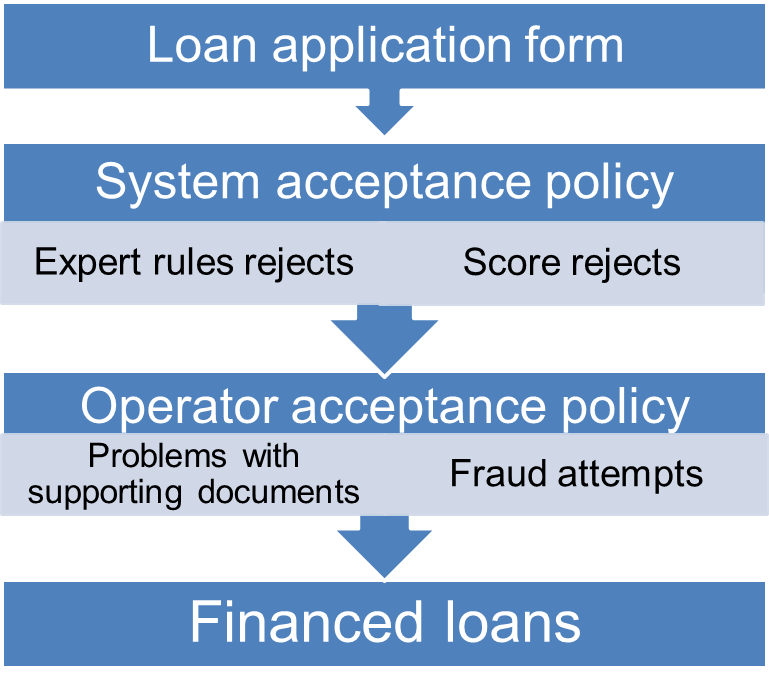
\includegraphics[width=5cm]{figures/schema.png}
\caption{Simplified financing mechanism in~Crédit Agricole Consumer Finance}
\label{fig:figure1}

\end{minipage}%
\hfil \begin{minipage}[c]{0.5\linewidth}

\center 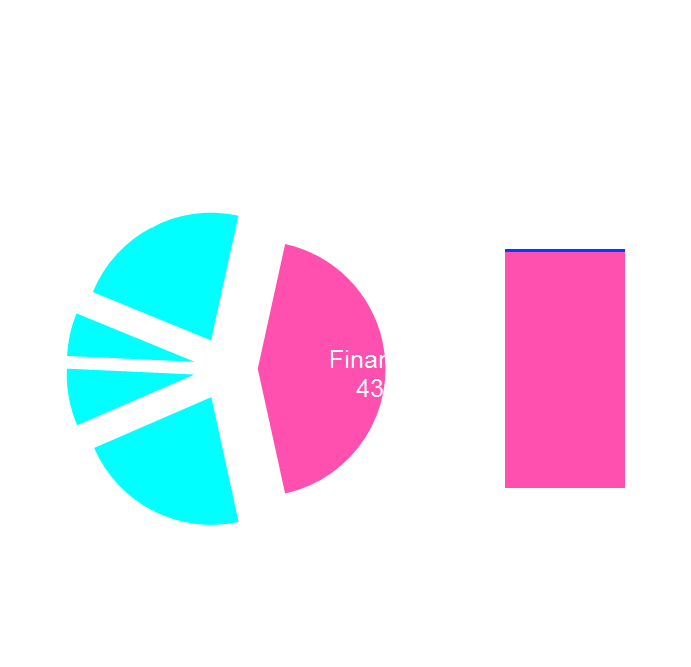
\includegraphics[width=5cm]{figures/camembert_invert.png}
\caption{Proportion of ``final'' lending decisions for CACF France}

\end{minipage}
\end{figure}

\end{frame}








\begin{frame}
\frametitle{\secname: \subsecname}

%%%%%%%%%%%%%%%%%%%%
\note{Si on revient à la formalisation statistique, on a une contrainte de modélisation par régression logistique, qu'on interprète ici comme un espace des paramètres grand $\theta$ fixe, et une pratique ``métier'' consistant à n'utiliser que les clients financés dans l'estimation de $\theta$ qu'on note $\hat{\bm{\theta}}_{\f}$.

\bigskip

A ce stade, implicitement, le chargé d'études statistiques approche un paramètre asymptotique symbolisé par l'étoile, minimisant une divergence de Kullback-Leibler entre la vraie loi et la loi logistique conditionnellement à Z=f, c-à-d au fait d'être financé.}
%%%%%%%%%%%%%%%%%%%%




The industry traditionally fits a logistic regression using only financed clients ({\bf fixed parameter space $\Theta$}):

\begin{minipage}[c]{0.1\linewidth}
\begin{animateinline}[autoplay,loop]{2}%
{\color{orange}{\bf CACF}}%
\newframe \end{animateinline}
\end{minipage}
\begin{minipage}[c]{0.85\linewidth}
\[ \hat{\bm{\theta}}_{\f} = \argmax_{\bm{\theta}} \ell(\bm{\theta} ; \mathcal{T}_\f) = \sum_{i=1}^n \ln p_{\bm{\theta}}(y_i | \bm{x}_i), \]
\end{minipage}
which asymptotically approximates:
\[ \bm{\theta}_{\f}^\star = \argmin_{\bm{\theta}} \mathbb{E}_{\bm{X}} [\text{KL}(p || p_{\bm{\theta}}) | Z = \f]. \]

\end{frame}





\begin{frame}
\frametitle{\secname: \subsecname}


%%%%%%%%%%%%%%%%%%%%%%%%
\note{Ce qu'on aimerait avoir plutôt, c'est le paramètre $\bm{\theta}^\star$ qui n'est pas conditionnel au fait d'être financé et qui pourrait être très simplement obtenu comme une quantité asymptotique du paramètre de maximum de vraisemblance $\hat{\bm{\theta}}$ irrémédiablement inaccessible puisqu'on ne connaît pas toutes les étiquettes.

D'un point de vue géométrique, on peut représenter l'espace des modèles de regression logistique de coefficient $\theta$, la vraie loi qui n'est pas forcément dans cet espace, le paramètre $\bm{\theta}^\star$ qui est la projection orthogonale de cette loi sur l'espace du modèle et le paramètre conditionnel au financement qui se promène dans cet espace et dont le biais est potentiellement plus grand que $\bm{\theta}^\star$.

C'est là tout l'enjeu d'une formalisation rigoureuse : montrer sous quelles hypothèses ce biais existe et si ces hypothèses sont réalistes.

Notons aussi que même à supposer que les paramètres asymptotiques sont égaux, la variance du paramètre conditionnel au fait d'être financé sera plus grande puisqu'on a moins d'observations.}
%%%%%%%%%%%%%%%%%%%%%%%%



Oracle to be approximated:
\begin{align*}
\bm{\theta}^\star & = \argmin_{\bm{\theta}} \mathbb{E}_{\bm{X}} [\text{KL}(p || p_{\bm{\theta}})] \\
& = \argmax_{\bm{\theta}} \mathbb{E}_{\bm{x}, y \sim p} [\ln p_{\bm{\theta}}(y | \bm{x})].
\end{align*}
which standard estimator would be:
\[ \hat{\bm{\theta}} = \argmax_{\bm{\theta}} \ell(\bm{\theta} ; \mathcal{T}_{\text{c}}), \]
But we lack $\mathbf{y}_{\nf}$.
\vspace*{-0.8cm}
\begin{center}
\resizebox{0.8\textwidth}{4.7cm}{
\begin{tikzpicture}[scale=1.1,every node/.style={minimum size=1cm},on grid]

	% Real level
	\begin{scope}[
		yshift=-120,
		every node/.append style={yslant=\yslant,xslant=\xslant},
		yslant=\yslant,xslant=\xslant
	] 
		% The frame:
		\draw[white, dashed, thin] (0,0) rectangle (7,7); 
		% Agents:
		\draw[fill=orange]  
			(5,2) circle (.1) % Firms
			(2,2) circle (.1); % Households
		% Flows:
		\draw[-latex,thin, yellow] 
			(2,2.2) to (2,4); % Labour Powers
		\draw[-latex,thin, yellow]
			(4.85,1.85) to (4,1); % Wages
		 % Labels:
		\fill[white]
			(0.5,6.5) node[right, scale=2.5] {Model space $\Theta$}	
			(4.9,1.9) node[right,scale=2]{$\theta_{\f}^\star$}
			(2.1,1.9) node[below,scale=2]{$\theta^\star$}
			(2.2,4.3) node [scale=2] {$\hat{\theta}$} 
			(4.2,0.6) node [scale=2] {$\hat{\theta}_{\f}$};
		\fill[yellow]
			(1,3) node [scale=1] {Estimation}
            (1,2.7) node [scale=1] {bias+variance};
		\fill[yellow]
			(5.7,1.1) node [scale=1] {Estimation}
            (5.7,0.8) node [scale=1] {bias+variance};

	\end{scope}
	
	% 2 vertical lines for linking agents on the 2 levels
	\draw[thin, dashed, orange](.8,1.75) to (3.8,-0.32);
	\draw[thin, dashed, orange](.8,1.75) to (.8,-1.8);
	
    % Draw right angle scheme
    \draw(.8,-1.6) to (1,-1.6);
    \draw(1,-1.6) to (1,-1.8);


	% Monetary level
	\begin{scope}[
		yshift=-20,
		every node/.append style={yslant=0,xslant=0},
		yslant=\yslant,xslant=\xslant
	]
		 % Agents:
		\draw [fill=green]
			(2,2) circle (.1); % Households
		 % Labels:
		\fill[black]
			(2.2,2.4) node[right,scale=2]{\textcolor{green}{$p(y|\bm{x})$}};
%			(4,2) node[right,scale=2]{\textcolor{olive}{$p(y|\bm{x}, z = \f)$}};
        \fill[orange]
			(0.85,0.35) node [right, scale=1.5] {Model bias};	

	\end{scope} 
\end{tikzpicture}
}
\end{center}


\end{frame}



\subsection{modelling the financing mechanism}

\begin{frame}
\frametitle{\secname : \subsecname}



%%%%%%%%%%%%%%
\note{}
%%%%%%%%%%%%%%

Due to the financing mechanism, labels $y$ are not MCAR.

\medskip

\uncover<2->{
Let $\{p_{\bm{\phi}}(z | \bm{x}, y)\}_{\bm{\phi} \in \bm{\Phi}}$ denote this hidden financing mechanism (as a parametrized family).
}

\medskip

\uncover<3->{
Combining financing and credit-worthiness probability distributions:
\[ p_{\bm{\gamma}}(y,z | \bm{x}) = p_{\bm{\theta}(\bm{\gamma})}(y | \bm{x}) p_{\bm{\phi}(\bm{\gamma})}(z | \bm{x}, y). \]
}

%\medskip

\uncover<4->{
To estimate $\bm{\gamma}$, we could rely on Maximum Likelihood theory.
}

\end{frame}



\begin{frame}
\frametitle{\secname : \subsecname}



%%%%%%%%%%%%%%
\note{}
%%%%%%%%%%%%%%

\begin{minipage}[c]{0.15\linewidth}
\begin{animateinline}[autoplay,loop]{2}%
{\color{orange}{\bf Statistician}}%
\newframe \end{animateinline}
\end{minipage}%
\begin{minipage}[c]{0.80\linewidth}
\[ \vspace*{-0.8cm} \hspace*{0.7cm} \ell(\bm{\gamma}; \mathcal{T}) = \sum_{i = 1}^n \ln p_{\bm{\gamma}}(y_i,\f | \bm{x}_i) + \sum_{i=n+1}^{n+n'} \ln \sum_{y \in \{0,1\}} p_{\bm{\gamma}}(y,\nf | \bm{x}_i), \]
\end{minipage}
\textit{e.g.}\ \textit{via} an EM algorithm:


\end{frame}






\subsection{missingness mechanism}

\begin{frame}
\frametitle{\secname : \subsecname}


%%%%%%%%%%%%%%%
\note{}
%%%%%%%%%%%%%%%



\begin{itemize}
\item \textbf{Ignorability}: no functional dependence between $\bm{\theta}$ and $\bm{\phi}$, \textit{e.g.}\ $\bm{\gamma} = (\bm{\theta},\bm{\phi})$.

\item<2-> \textbf{MAR}: $\forall \: \bm{x},y,z, \; p(z| \bm{x},y) = p(z| \bm{x})$

$\rightarrow$ Financing is determined by an old score: $Z = \mathds{1}_{\{\bm{\theta}'X > \text{cut}\}}$.

\item<3-> \textbf{MNAR}: $\exists \: \bm{x},y,z, \; p(z| \bm{x},y) \neq p(z| \bm{x})$

$\rightarrow$ Operators' hidden ``feeling'' features $\tilde{\bm{X}}$ influence the financing.

$\rightarrow$ Expert rules based on both present and hidden features $\bm{X}$ and $\tilde{\bm{X}}$ resp.\ where $\tilde{\bm{X}}$ cannot be totally explained by $\bm{X}$.
\end{itemize}

\uncover<4->{
\begin{figure}
\begin{tikzpicture}

\tikzset{vertex/.style = {shape=circle,draw,minimum size=1.5em}}
\tikzset{edge/.style = {->,> = latex'}}
% vertices
\node[vertex] (y) at  (0,0) {$Y$};
\node[vertex] (x) at  (2,-1) {$\bm{X}$};
\node[vertex] (xc) at  (2,1) {$\tilde{\bm{X}}$};
\node[vertex] (z) at (4,0) {$Z$};

edges
\draw[edge] (y) to (x);
\draw[edge] (y) to (xc);
\draw[dashed] (xc) to (x);
\draw[edge] (xc) to (z);
\draw[edge] (x) to (z);

\end{tikzpicture}
\label{fig:mar}
\caption{Dependencies between random variables $Y$, $\bm{\tilde{X}}$, $\bm{X}$ and $Z$}
\end{figure}
}
\end{frame}




\subsection{flawed model selection}

\begin{frame}
\frametitle{\secname : \subsecname}



%%%%%%%%%%%
\note{}
%%%%%%%%%%%



Because no test-sample $\mathcal{T}^{\text{test}}$ is available from $p(\bm{x}, y, z)$, we cannot resort to error-rate criteria.

\medskip

\uncover<2->{
We should use information criteria on the observed data $\mathcal{T}$ such as:
\[ \text{BIC}(\hat{\bm{\gamma}};\mathcal{T}) = -2 \ell(\hat{\bm{\gamma}}; \mathcal{T}) + \text{dim}(\bm{\Gamma})\ln n, \]
where $\hat{\bm{\gamma}} = \argmax_{\bm{\gamma}} \ell(\bm{\gamma}; \mathcal{T})$, to compare models.
}

\medskip

\uncover<3->{
It requires to precisely state the models $\{ p_{\bm{\gamma}}(y,z | \bm{x})\}_{\bm{\Gamma}}$ that compete and underlying assumptions.
}

\end{frame}



\subsection{reject inference strategies}

\begin{frame}
\frametitle{\secname : \subsecname}



%%%%%%%%%%%%%%%%
\note{}
%%%%%%%%%%%%%%%%




We gathered 6 so-called Reject Inference methods from the literature~\cite{economix,saporta,RI6,banasik} that aim at re-injecting $\bm{\mathbf{x}}_{\nf}$ into the estimation procedure of $\bm{\theta}$.

\medskip

They usually resemble EM-like algorithms:

{
\setbeamercolor{normal text}{fg=black}
\usebeamercolor[fg]{normal text}

\[ \hspace*{-0.8cm}\textcolor{white}{\mathcal{T}_{\text{c}}^{(1)} = {\Huge \Bigg(}}
%\begin{array}{c}
%\tikzmarkin[hor=style green]{el0} \mathbf{x}_{\f} \tikzmarkend{el0} \\
%\\
%\\
%\tikzmarkin[hor=style green]{el-1} \mathbf{x}_{\nf} \tikzmarkend{el-1} \end{array}
\textcolor{white}{{\Huge \Bigg(}}
\begin{array}{ccc}
\tikzmarkin[hor=style green]{el1} \; \; x_{1,1} & \cdots & x_{1,d}  \\
 \vdots & \vdots & \vdots \\
 x_{n,1} & \cdots & x_{n,d} \\
 x_{n+1,1} & \cdots & x_{n+1,d}  \\
 \vdots & \vdots & \vdots \\
 x_{n+n',1} & \cdots & x_{n+n',d} \tikzmarkend{el1} \end{array} \textcolor{white}{{\Huge \Bigg)},}
 %\hspace{0.2cm}
% \begin{array}{c}
%\tikzmarkin[hor=style green]{l1} \mathbf{y}_{\f} \tikzmarkend{l1}\\
%\\
%\\
%\tikzmarkin[hor=style green]{l2} \mathbf{y}_{\nf} \tikzmarkend{l2} \end{array}
\textcolor{white}{{\Huge \Bigg(}}
\begin{array}{c}
\tikzmarkin[hor=style green]{l3} \; \; y_1 \; \; \; \\
\vdots \\
 y_n \\ 
 \hat{y}_{n+1}^{(1)} \\
\vdots \\
\hat{y}_{n+n'}^{(1)} \tikzmarkend{l3}\end{array} \textcolor{white}{{\Huge \Bigg)},}
%\hspace{0.2cm} 
% \begin{array}{c}
%\tikzmarkin[hor=style green]{el111} \mathbf{z}_{\f} \tikzmarkend{el111}\\
%\\
%\\
%\tikzmarkin[hor=style green]{el121} \mathbf{z}_{\nf} \tikzmarkend{el121}\end{array}
\textcolor{white}{{\Huge \Bigg(}}
\begin{array}{c}
\tikzmarkin[hor=style green]{e41} \text{f} \\
\vdots \\
\text{f} \\ 
\text{nf} \\
\vdots \\
\text{nf} \tikzmarkend{e41} \end{array} \textcolor{white}{{\Huge \Bigg) \Bigg)}}\]
 }
 
%\setbeamercolor{normal text}{fg=white}
%\usebeamercolor[fg]{normal text}

\end{frame}



\subsection{theoretical findings}

\begin{frame}
\frametitle{\secname : \subsecname}


%%%%%%%%%%%%%%%%
\note{}
%%%%%%%%%%%%%%%%




Fuzzy augmentation and Twins produce the same coefficient $\hat{\bm{\theta}}_{\text{f}}$.

\medskip

Reclassification is equivalent to a Classification-EM algorithm, thus introducing a bias in the estimation of $\bm{\theta}$.

\begin{table}
\caption{Summary of potential biases.}
\begin{center}
\begin{tabular}{L{2cm} | C{4cm} | C{4cm}}
 & MAR & MNAR \\
 \hline
 Well-specified model & $\hat{\bm{\theta}}_{\text{f}}$ is asymptotically unbiased. & \multirowcell{2}{$\hat{\bm{\theta}}_{\text{f}}$ is asymptotically \\ biased. Any correction  \\ relies on \textit{a priori} \\ unverifiable assumptions \\ about $p_{\bm{\phi}}(z | \bm{x}, y)$.} \\
 \cline{1-2}
 Misspecified model & $\hat{\bm{\theta}}_{\text{f}}$ is asymptotically biased: the Augmentation method could be suitable but introduces a new estimation procedure. & \\
\end{tabular}
\end{center}
\end{table}

\end{frame}



\subsection{some simulations}

\begin{frame}
\frametitle{\secname : \subsecname}



%%%%%%%%%%%%%%%%
\note{On retourne au cadre CACF où on teste ces trois méthodes sur deux jeux de données : un portefeuille d'un partenaire de grande distribution et un portefeuille compte propre, c-à-d Sofinco

\bigskip

Dans les deux cas, on simule artificiellement un mécanisme de rejet en augmentant progressivement le cut de l'ancien score, jusqu'au point où il n'y a plus suffisamment de mauvais payeur pour apprendre.

\bigskip

On a ainsi une sorte d'ensemble test de $p(x,y,z)$.

\bigskip

On remarque que les trois méthodes ne sont pas significativement différentes en termes de Gini.

\bigskip

Notre conseil à CACF est donc de ne pas pratiquer de réintégration dans le cas de la régression logistique.
}
%%%%%%%%%%%%%%%%



\vspace*{-1cm}
\begin{figure}[!ht]
\centering \resizebox{\textwidth}{!}{% Created by tikzDevice version 0.12 on 2019-06-13 15:42:19
% !TEX encoding = UTF-8 Unicode
\begin{tikzpicture}[x=1pt,y=1pt, scale=0.6]
\definecolor{fillColor}{RGB}{255,255,255}
\path[use as bounding box,fill=fillColor,fill opacity=0.00] (0,0) rectangle (578.16,231.26);
\begin{scope}
\path[clip] ( 49.20, 61.20) rectangle (552.96,182.06);
\definecolor{drawColor}{RGB}{255,255,255}

\path[draw=drawColor,line width= 1.2pt,line join=round,line cap=round] ( 67.86,176.85) --
	( 67.90,176.85) --
	( 67.90,176.85) --
	(108.35,176.26) --
	(122.20,177.56) --
	(201.20,177.59) --
	(291.41,156.62) --
	(349.16,151.14) --
	(432.12,114.79) --
	(518.48, 65.68);
\definecolor{fillColor}{RGB}{255,255,255}

\path[fill=fillColor] ( 65.61,174.60) --
	( 70.11,174.60) --
	( 70.11,179.10) --
	( 65.61,179.10) --
	cycle;

\path[fill=fillColor] ( 65.65,174.60) --
	( 70.15,174.60) --
	( 70.15,179.10) --
	( 65.65,179.10) --
	cycle;

\path[fill=fillColor] ( 65.65,174.60) --
	( 70.15,174.60) --
	( 70.15,179.10) --
	( 65.65,179.10) --
	cycle;

\path[fill=fillColor] (106.10,174.01) --
	(110.60,174.01) --
	(110.60,178.51) --
	(106.10,178.51) --
	cycle;

\path[fill=fillColor] (119.95,175.31) --
	(124.45,175.31) --
	(124.45,179.81) --
	(119.95,179.81) --
	cycle;

\path[fill=fillColor] (198.95,175.34) --
	(203.45,175.34) --
	(203.45,179.84) --
	(198.95,179.84) --
	cycle;

\path[fill=fillColor] (289.16,154.37) --
	(293.66,154.37) --
	(293.66,158.87) --
	(289.16,158.87) --
	cycle;

\path[fill=fillColor] (346.91,148.89) --
	(351.41,148.89) --
	(351.41,153.39) --
	(346.91,153.39) --
	cycle;

\path[fill=fillColor] (429.87,112.54) --
	(434.37,112.54) --
	(434.37,117.04) --
	(429.87,117.04) --
	cycle;

\path[fill=fillColor] (516.23, 63.43) --
	(520.73, 63.43) --
	(520.73, 67.93) --
	(516.23, 67.93) --
	cycle;
\end{scope}
\begin{scope}
\path[clip] (  0.00,  0.00) rectangle (578.16,231.26);
\definecolor{drawColor}{RGB}{255,255,255}

\path[draw=drawColor,line width= 1.2pt,line join=round,line cap=round] ( 49.20, 61.20) --
	(552.96, 61.20) --
	(552.96,182.06) --
	( 49.20,182.06) --
	( 49.20, 61.20);
\end{scope}
\begin{scope}
\path[clip] (  0.00,  0.00) rectangle (578.16,231.26);
\definecolor{drawColor}{RGB}{255,255,255}

\node[text=drawColor,anchor=base,inner sep=0pt, outer sep=0pt, scale=  1.00] at (301.08, 15.60) {Acceptance rate};

\node[text=drawColor,rotate= 90.00,anchor=base,inner sep=0pt, outer sep=0pt, scale=  1.00] at ( 10.80,121.63) {Gini on test set};
\end{scope}
\begin{scope}
\path[clip] ( 49.20, 61.20) rectangle (552.96,182.06);
\definecolor{drawColor}{RGB}{255,165,0}

\path[draw=drawColor,line width= 1.2pt,dash pattern=on 1pt off 3pt ,line join=round,line cap=round] ( 67.86,177.22) --
	( 67.90,177.22) --
	( 67.90,177.22) --
	(108.35,175.71) --
	(122.20,176.52) --
	(201.20,177.59) --
	(291.41,152.44) --
	(349.16,151.70) --
	(432.12,116.95) --
	(518.48, 65.68);
\definecolor{fillColor}{RGB}{255,165,0}

\path[fill=fillColor] ( 67.86,180.72) --
	( 70.89,175.48) --
	( 64.83,175.48) --
	cycle;

\path[fill=fillColor] ( 67.90,180.72) --
	( 70.93,175.48) --
	( 64.87,175.48) --
	cycle;

\path[fill=fillColor] ( 67.90,180.72) --
	( 70.93,175.48) --
	( 64.87,175.48) --
	cycle;

\path[fill=fillColor] (108.35,179.21) --
	(111.38,173.96) --
	(105.32,173.96) --
	cycle;

\path[fill=fillColor] (122.20,180.02) --
	(125.23,174.77) --
	(119.17,174.77) --
	cycle;

\path[fill=fillColor] (201.20,181.09) --
	(204.23,175.84) --
	(198.17,175.84) --
	cycle;

\path[fill=fillColor] (291.41,155.94) --
	(294.45,150.69) --
	(288.38,150.69) --
	cycle;

\path[fill=fillColor] (349.16,155.20) --
	(352.19,149.95) --
	(346.13,149.95) --
	cycle;

\path[fill=fillColor] (432.12,120.45) --
	(435.15,115.20) --
	(429.09,115.20) --
	cycle;

\path[fill=fillColor] (518.48, 69.18) --
	(521.51, 63.93) --
	(515.45, 63.93) --
	cycle;
\end{scope}
\begin{scope}
\path[clip] (  0.00,  0.00) rectangle (578.16,231.26);
\definecolor{drawColor}{RGB}{255,255,255}

\path[draw=drawColor,line width= 1.2pt,line join=round,line cap=round] ( 49.20, 61.20) --
	(552.96, 61.20) --
	(552.96,182.06) --
	( 49.20,182.06) --
	( 49.20, 61.20);
\end{scope}
\begin{scope}
\path[clip] (  0.00,  0.00) rectangle (578.16,231.26);
\definecolor{drawColor}{RGB}{255,255,255}

\node[text=drawColor,anchor=base,inner sep=0pt, outer sep=0pt, scale=  1.00] at (301.08, 15.60) {Acceptance rate};

\node[text=drawColor,rotate= 90.00,anchor=base,inner sep=0pt, outer sep=0pt, scale=  1.00] at ( 10.80,121.63) {Gini on test set};
\end{scope}
\begin{scope}
\path[clip] ( 49.20, 61.20) rectangle (552.96,182.06);
\definecolor{drawColor}{RGB}{255,0,255}

\path[draw=drawColor,line width= 1.2pt,dash pattern=on 1pt off 3pt on 4pt off 3pt ,line join=round,line cap=round] ( 67.86,177.59) --
	( 67.90,177.59) --
	( 67.90,177.59) --
	(108.35,176.27) --
	(122.20,176.39) --
	(201.20,176.36) --
	(291.41,156.29) --
	(349.16,162.21) --
	(432.12,108.61) --
	(518.48, 65.68);

\path[draw=drawColor,line width= 1.2pt,line join=round,line cap=round] ( 65.61,175.34) -- ( 70.11,179.84);

\path[draw=drawColor,line width= 1.2pt,line join=round,line cap=round] ( 65.61,179.84) -- ( 70.11,175.34);

\path[draw=drawColor,line width= 1.2pt,line join=round,line cap=round] ( 64.68,177.59) -- ( 71.04,177.59);

\path[draw=drawColor,line width= 1.2pt,line join=round,line cap=round] ( 67.86,174.41) -- ( 67.86,180.77);

\path[draw=drawColor,line width= 1.2pt,line join=round,line cap=round] ( 65.65,175.34) -- ( 70.15,179.84);

\path[draw=drawColor,line width= 1.2pt,line join=round,line cap=round] ( 65.65,179.84) -- ( 70.15,175.34);

\path[draw=drawColor,line width= 1.2pt,line join=round,line cap=round] ( 64.71,177.59) -- ( 71.08,177.59);

\path[draw=drawColor,line width= 1.2pt,line join=round,line cap=round] ( 67.90,174.41) -- ( 67.90,180.77);

\path[draw=drawColor,line width= 1.2pt,line join=round,line cap=round] ( 65.65,175.34) -- ( 70.15,179.84);

\path[draw=drawColor,line width= 1.2pt,line join=round,line cap=round] ( 65.65,179.84) -- ( 70.15,175.34);

\path[draw=drawColor,line width= 1.2pt,line join=round,line cap=round] ( 64.71,177.59) -- ( 71.08,177.59);

\path[draw=drawColor,line width= 1.2pt,line join=round,line cap=round] ( 67.90,174.41) -- ( 67.90,180.77);

\path[draw=drawColor,line width= 1.2pt,line join=round,line cap=round] (106.10,174.02) -- (110.60,178.52);

\path[draw=drawColor,line width= 1.2pt,line join=round,line cap=round] (106.10,178.52) -- (110.60,174.02);

\path[draw=drawColor,line width= 1.2pt,line join=round,line cap=round] (105.17,176.27) -- (111.53,176.27);

\path[draw=drawColor,line width= 1.2pt,line join=round,line cap=round] (108.35,173.09) -- (108.35,179.45);

\path[draw=drawColor,line width= 1.2pt,line join=round,line cap=round] (119.95,174.14) -- (124.45,178.64);

\path[draw=drawColor,line width= 1.2pt,line join=round,line cap=round] (119.95,178.64) -- (124.45,174.14);

\path[draw=drawColor,line width= 1.2pt,line join=round,line cap=round] (119.02,176.39) -- (125.38,176.39);

\path[draw=drawColor,line width= 1.2pt,line join=round,line cap=round] (122.20,173.21) -- (122.20,179.57);

\path[draw=drawColor,line width= 1.2pt,line join=round,line cap=round] (198.95,174.11) -- (203.45,178.61);

\path[draw=drawColor,line width= 1.2pt,line join=round,line cap=round] (198.95,178.61) -- (203.45,174.11);

\path[draw=drawColor,line width= 1.2pt,line join=round,line cap=round] (198.02,176.36) -- (204.38,176.36);

\path[draw=drawColor,line width= 1.2pt,line join=round,line cap=round] (201.20,173.18) -- (201.20,179.54);

\path[draw=drawColor,line width= 1.2pt,line join=round,line cap=round] (289.16,154.04) -- (293.66,158.54);

\path[draw=drawColor,line width= 1.2pt,line join=round,line cap=round] (289.16,158.54) -- (293.66,154.04);

\path[draw=drawColor,line width= 1.2pt,line join=round,line cap=round] (288.23,156.29) -- (294.60,156.29);

\path[draw=drawColor,line width= 1.2pt,line join=round,line cap=round] (291.41,153.11) -- (291.41,159.48);

\path[draw=drawColor,line width= 1.2pt,line join=round,line cap=round] (346.91,159.96) -- (351.41,164.46);

\path[draw=drawColor,line width= 1.2pt,line join=round,line cap=round] (346.91,164.46) -- (351.41,159.96);

\path[draw=drawColor,line width= 1.2pt,line join=round,line cap=round] (345.98,162.21) -- (352.34,162.21);

\path[draw=drawColor,line width= 1.2pt,line join=round,line cap=round] (349.16,159.03) -- (349.16,165.39);

\path[draw=drawColor,line width= 1.2pt,line join=round,line cap=round] (429.87,106.36) -- (434.37,110.86);

\path[draw=drawColor,line width= 1.2pt,line join=round,line cap=round] (429.87,110.86) -- (434.37,106.36);

\path[draw=drawColor,line width= 1.2pt,line join=round,line cap=round] (428.94,108.61) -- (435.31,108.61);

\path[draw=drawColor,line width= 1.2pt,line join=round,line cap=round] (432.12,105.43) -- (432.12,111.79);

\path[draw=drawColor,line width= 1.2pt,line join=round,line cap=round] (516.23, 63.43) -- (520.73, 67.93);

\path[draw=drawColor,line width= 1.2pt,line join=round,line cap=round] (516.23, 67.93) -- (520.73, 63.43);

\path[draw=drawColor,line width= 1.2pt,line join=round,line cap=round] (515.30, 65.68) -- (521.66, 65.68);

\path[draw=drawColor,line width= 1.2pt,line join=round,line cap=round] (518.48, 62.49) -- (518.48, 68.86);
\end{scope}
\begin{scope}
\path[clip] (  0.00,  0.00) rectangle (578.16,231.26);
\definecolor{drawColor}{RGB}{255,255,255}

\path[draw=drawColor,line width= 1.2pt,line join=round,line cap=round] ( 49.20, 61.20) --
	(552.96, 61.20) --
	(552.96,182.06) --
	( 49.20,182.06) --
	( 49.20, 61.20);
\end{scope}
\begin{scope}
\path[clip] (  0.00,  0.00) rectangle (578.16,231.26);
\definecolor{drawColor}{RGB}{255,255,255}

\node[text=drawColor,anchor=base,inner sep=0pt, outer sep=0pt, scale=  1.00] at (301.08, 15.60) {Acceptance rate};

\node[text=drawColor,rotate= 90.00,anchor=base,inner sep=0pt, outer sep=0pt, scale=  1.00] at ( 10.80,121.63) {Gini on test set};
\end{scope}
\begin{scope}
\path[clip] (  0.00,  0.00) rectangle (578.16,231.26);
\definecolor{drawColor}{RGB}{255,255,255}

\path[draw=drawColor,line width= 1.2pt,line join=round,line cap=round] (534.30, 61.20) -- ( 67.86, 61.20);

\path[draw=drawColor,line width= 1.2pt,line join=round,line cap=round] (534.30, 61.20) -- (534.30, 55.20);
\node[text=drawColor,anchor=base east,inner sep=0pt, outer sep=0pt, scale=  1.00] at (550, 45) {60 \%};

\path[draw=drawColor,line width= 1.2pt,line join=round,line cap=round] (417.69, 61.20) -- (417.69, 55.20);
\node[text=drawColor,anchor=base east,inner sep=0pt, outer sep=0pt, scale=  1.00] at (430, 45) {70 \%};

\path[draw=drawColor,line width= 1.2pt,line join=round,line cap=round] (301.08, 61.20) -- (301.08, 55.20);
\node[text=drawColor,anchor=base east,inner sep=0pt, outer sep=0pt, scale=  1.00] at (315, 45) {80 \%};

\path[draw=drawColor,line width= 1.2pt,line join=round,line cap=round] (184.47, 61.20) -- (184.47, 55.20);
\node[text=drawColor,anchor=base east,inner sep=0pt, outer sep=0pt, scale=  1.00] at (200, 45) {90 \%};

\path[draw=drawColor,line width= 1.2pt,line join=round,line cap=round] ( 67.86, 61.20) -- ( 67.86, 55.20);
\node[text=drawColor,anchor=base east,inner sep=0pt, outer sep=0pt, scale=  1.00] at (80, 45) {100 \%};


%\path[draw=drawColor,line width= 1.2pt,line join=round,line cap=round] ( 49.20, 17.92) -- ( 49.20,210.29);

\path[draw=drawColor,line width= 1.2pt,line join=round,line cap=round] ( 49.20, 61.20) -- ( 49.20,182.06);

%\path[draw=drawColor,line width= 1.2pt,line join=round,line cap=round] ( 49.20, 17.92) -- ( 43.20, 17.92);

%\path[draw=drawColor,line width= 1.2pt,line join=round,line cap=round] ( 49.20, 49.98) -- ( 43.20, 49.98);

\path[draw=drawColor,line width= 1.2pt,line join=round,line cap=round] ( 49.20, 82.04) -- ( 43.20, 82.04);

\path[draw=drawColor,line width= 1.2pt,line join=round,line cap=round] ( 49.20,114.10) -- ( 43.20,114.10);

\path[draw=drawColor,line width= 1.2pt,line join=round,line cap=round] ( 49.20,146.17) -- ( 43.20,146.17);

\path[draw=drawColor,line width= 1.2pt,line join=round,line cap=round] ( 49.20,178.23) -- ( 43.20,178.23);

%\path[draw=drawColor,line width= 1.2pt,line join=round,line cap=round] ( 49.20,210.29) -- ( 43.20,210.29);

%\node[text=drawColor,anchor=base east,inner sep=0pt, outer sep=0pt, scale=  1.00] at ( 37.20, 14.47) {-10};

%\node[text=drawColor,anchor=base east,inner sep=0pt, outer sep=0pt, scale=  1.00] at ( 37.20, 46.54) {0};

\node[text=drawColor,anchor=base east,inner sep=0pt, outer sep=0pt, scale=  1.00] at ( 37.20, 78.60) {10};

\node[text=drawColor,anchor=base east,inner sep=0pt, outer sep=0pt, scale=  1.00] at ( 37.20,110.66) {20};

\node[text=drawColor,anchor=base east,inner sep=0pt, outer sep=0pt, scale=  1.00] at ( 37.20,142.72) {30};

\node[text=drawColor,anchor=base east,inner sep=0pt, outer sep=0pt, scale=  1.00] at ( 37.20,174.79) {40};

%\node[text=drawColor,anchor=base east,inner sep=0pt, outer sep=0pt, scale=  1.00] at ( 37.20,206.85) {50};

\path[draw=drawColor,line width= 1.2pt,line join=round,line cap=round] ( 67.86,155.79) rectangle (180.16,119.79);

\path[draw=drawColor,line width= 1.2pt,line join=round,line cap=round] ( 69.88,146.79) -- ( 83.38,146.79);
\definecolor{drawColor}{RGB}{255,165,0}

\path[draw=drawColor,line width= 1.2pt,dash pattern=on 1pt off 3pt ,line join=round,line cap=round] ( 69.88,137.79) -- ( 83.38,137.79);
\definecolor{drawColor}{RGB}{255,0,255}

\path[draw=drawColor,line width= 1.2pt,dash pattern=on 1pt off 3pt on 4pt off 3pt ,line join=round,line cap=round] ( 69.88,128.79) -- ( 83.38,128.79);
\definecolor{fillColor}{RGB}{255,255,255}

\path[fill=fillColor] ( 74.95,145.10) --
	( 78.32,145.10) --
	( 78.32,148.47) --
	( 74.95,148.47) --
	cycle;
\definecolor{fillColor}{RGB}{255,165,0}

\path[fill=fillColor] ( 76.63,140.41) --
	( 78.91,136.47) --
	( 74.36,136.47) --
	cycle;

\path[draw=drawColor,line width= 1.2pt,line join=round,line cap=round] ( 74.95,127.10) -- ( 78.32,130.47);

\path[draw=drawColor,line width= 1.2pt,line join=round,line cap=round] ( 74.95,130.47) -- ( 78.32,127.10);

\path[draw=drawColor,line width= 1.2pt,line join=round,line cap=round] ( 74.25,128.79) -- ( 79.02,128.79);

\path[draw=drawColor,line width= 1.2pt,line join=round,line cap=round] ( 76.63,126.40) -- ( 76.63,131.17);
\definecolor{drawColor}{RGB}{255,255,255}

\node[text=drawColor,anchor=base west,inner sep=0pt, outer sep=0pt, scale=  0.75] at ( 90.13,144.20) {Financed};

\node[text=drawColor,anchor=base west,inner sep=0pt, outer sep=0pt, scale=  0.75] at ( 90.13,135.20) {Augmentation};

\node[text=drawColor,anchor=base west,inner sep=0pt, outer sep=0pt, scale=  0.75] at ( 90.13,126.20) {Parcelling};
\end{scope}
\end{tikzpicture}
}
%\caption{Electronics loans dataset from CACF.}
%\label{fig:darty_reject}
\end{figure}
\vspace*{-1.5cm}
\begin{figure}[!ht]
\centering \resizebox{\textwidth}{!}{% Created by tikzDevice version 0.12 on 2019-06-13 08:41:07
% !TEX encoding = UTF-8 Unicode
\begin{tikzpicture}[x=1pt,y=1pt, scale=0.6]
\definecolor{fillColor}{RGB}{255,255,255}
\path[use as bounding box,fill=fillColor,fill opacity=0.00] (0,0) rectangle (578.16,231.26);
\begin{scope}
\path[clip] ( 49.20, 61.20) rectangle (552.96,182.06);
\definecolor{drawColor}{RGB}{255,255,255}

\path[draw=drawColor,line width= 1.2pt,line join=round,line cap=round] ( 67.86,162.53) --
	( 69.08,162.33) --
	(103.45,162.95) --
	(152.47,162.52) --
	(206.06,156.60) --
	(261.35,156.53) --
	(315.48,146.87) --
	(420.33,110.83) --
	(538.69, 70.37);
\definecolor{fillColor}{RGB}{255,255,255}

\path[fill=fillColor] ( 65.61,160.28) --
	( 70.11,160.28) --
	( 70.11,164.78) --
	( 65.61,164.78) --
	cycle;

\path[fill=fillColor] ( 66.83,160.08) --
	( 71.33,160.08) --
	( 71.33,164.58) --
	( 66.83,164.58) --
	cycle;

\path[fill=fillColor] (101.20,160.70) --
	(105.70,160.70) --
	(105.70,165.20) --
	(101.20,165.20) --
	cycle;

\path[fill=fillColor] (150.22,160.27) --
	(154.72,160.27) --
	(154.72,164.77) --
	(150.22,164.77) --
	cycle;

\path[fill=fillColor] (203.81,154.35) --
	(208.31,154.35) --
	(208.31,158.85) --
	(203.81,158.85) --
	cycle;

\path[fill=fillColor] (259.10,154.28) --
	(263.60,154.28) --
	(263.60,158.78) --
	(259.10,158.78) --
	cycle;

\path[fill=fillColor] (313.23,144.62) --
	(317.73,144.62) --
	(317.73,149.12) --
	(313.23,149.12) --
	cycle;

\path[fill=fillColor] (418.08,108.58) --
	(422.58,108.58) --
	(422.58,113.08) --
	(418.08,113.08) --
	cycle;

\path[fill=fillColor] (536.44, 68.12) --
	(540.94, 68.12) --
	(540.94, 72.62) --
	(536.44, 72.62) --
	cycle;
\end{scope}
\begin{scope}
\path[clip] (  0.00,  0.00) rectangle (578.16,231.26);
\definecolor{drawColor}{RGB}{255,255,255}

\path[draw=drawColor,line width= 1.2pt,line join=round,line cap=round] ( 49.20, 61.20) --
	(552.96, 61.20) --
	(552.96,182.06) --
	( 49.20,182.06) --
	( 49.20, 61.20);
\end{scope}
\begin{scope}
\path[clip] (  0.00,  0.00) rectangle (578.16,231.26);
\definecolor{drawColor}{RGB}{255,255,255}

\node[text=drawColor,anchor=base,inner sep=0pt, outer sep=0pt, scale=  1.00] at (301.08, 15.60) {Acceptance rate};

\node[text=drawColor,rotate= 90.00,anchor=base,inner sep=0pt, outer sep=0pt, scale=  1.00] at ( 10.80,121.63) {Gini on test set};
\end{scope}
\begin{scope}
\path[clip] ( 49.20, 61.20) rectangle (552.96,182.06);
\definecolor{drawColor}{RGB}{255,165,0}

\path[draw=drawColor,line width= 1.2pt,dash pattern=on 1pt off 3pt ,line join=round,line cap=round] ( 67.86,162.53) --
	( 69.08,162.35) --
	(103.45,161.79) --
	(152.47,162.52) --
	(206.06,155.98) --
	(261.35,159.22) --
	(315.48,146.34) --
	(420.33,109.94) --
	(538.69, 70.37);
\definecolor{fillColor}{RGB}{255,165,0}

\path[fill=fillColor] ( 67.86,166.03) --
	( 70.89,160.78) --
	( 64.83,160.78) --
	cycle;

\path[fill=fillColor] ( 69.08,165.85) --
	( 72.11,160.60) --
	( 66.05,160.60) --
	cycle;

\path[fill=fillColor] (103.45,165.29) --
	(106.48,160.04) --
	(100.42,160.04) --
	cycle;

\path[fill=fillColor] (152.47,166.01) --
	(155.50,160.77) --
	(149.44,160.77) --
	cycle;

\path[fill=fillColor] (206.06,159.48) --
	(209.09,154.23) --
	(203.03,154.23) --
	cycle;

\path[fill=fillColor] (261.35,162.72) --
	(264.38,157.47) --
	(258.32,157.47) --
	cycle;

\path[fill=fillColor] (315.48,149.84) --
	(318.51,144.60) --
	(312.45,144.60) --
	cycle;

\path[fill=fillColor] (420.33,113.44) --
	(423.36,108.20) --
	(417.30,108.20) --
	cycle;

\path[fill=fillColor] (538.69, 73.87) --
	(541.72, 68.62) --
	(535.66, 68.62) --
	cycle;
\end{scope}
\begin{scope}
\path[clip] (  0.00,  0.00) rectangle (578.16,231.26);
\definecolor{drawColor}{RGB}{255,255,255}

\path[draw=drawColor,line width= 1.2pt,line join=round,line cap=round] ( 49.20, 61.20) --
	(552.96, 61.20) --
	(552.96,182.06) --
	( 49.20,182.06) --
	( 49.20, 61.20);
\end{scope}
\begin{scope}
\path[clip] (  0.00,  0.00) rectangle (578.16,231.26);
\definecolor{drawColor}{RGB}{255,255,255}

\node[text=drawColor,anchor=base,inner sep=0pt, outer sep=0pt, scale=  1.00] at (301.08, 15.60) {Acceptance rate};

\node[text=drawColor,rotate= 90.00,anchor=base,inner sep=0pt, outer sep=0pt, scale=  1.00] at ( 10.80,121.63) {Gini on test set};
\end{scope}
\begin{scope}
\path[clip] ( 49.20, 61.20) rectangle (552.96,182.06);
\definecolor{drawColor}{RGB}{255,0,255}

\path[draw=drawColor,line width= 1.2pt,dash pattern=on 1pt off 3pt on 4pt off 3pt ,line join=round,line cap=round] ( 67.86,162.53) --
	( 69.08,162.05) --
	(103.45,161.39) --
	(152.47,162.52) --
	(206.06,152.75) --
	(261.35,155.28) --
	(315.48,152.27) --
	(420.33,164.74) --
	(538.69, 70.37);

\path[draw=drawColor,line width= 1.2pt,line join=round,line cap=round] ( 65.61,160.28) -- ( 70.11,164.78);

\path[draw=drawColor,line width= 1.2pt,line join=round,line cap=round] ( 65.61,164.78) -- ( 70.11,160.28);

\path[draw=drawColor,line width= 1.2pt,line join=round,line cap=round] ( 64.68,162.53) -- ( 71.04,162.53);

\path[draw=drawColor,line width= 1.2pt,line join=round,line cap=round] ( 67.86,159.35) -- ( 67.86,165.71);

\path[draw=drawColor,line width= 1.2pt,line join=round,line cap=round] ( 66.83,159.80) -- ( 71.33,164.30);

\path[draw=drawColor,line width= 1.2pt,line join=round,line cap=round] ( 66.83,164.30) -- ( 71.33,159.80);

\path[draw=drawColor,line width= 1.2pt,line join=round,line cap=round] ( 65.90,162.05) -- ( 72.26,162.05);

\path[draw=drawColor,line width= 1.2pt,line join=round,line cap=round] ( 69.08,158.87) -- ( 69.08,165.23);

\path[draw=drawColor,line width= 1.2pt,line join=round,line cap=round] (101.20,159.14) -- (105.70,163.64);

\path[draw=drawColor,line width= 1.2pt,line join=round,line cap=round] (101.20,163.64) -- (105.70,159.14);

\path[draw=drawColor,line width= 1.2pt,line join=round,line cap=round] (100.27,161.39) -- (106.63,161.39);

\path[draw=drawColor,line width= 1.2pt,line join=round,line cap=round] (103.45,158.21) -- (103.45,164.57);

\path[draw=drawColor,line width= 1.2pt,line join=round,line cap=round] (150.22,160.27) -- (154.72,164.77);

\path[draw=drawColor,line width= 1.2pt,line join=round,line cap=round] (150.22,164.77) -- (154.72,160.27);

\path[draw=drawColor,line width= 1.2pt,line join=round,line cap=round] (149.29,162.52) -- (155.65,162.52);

\path[draw=drawColor,line width= 1.2pt,line join=round,line cap=round] (152.47,159.33) -- (152.47,165.70);

\path[draw=drawColor,line width= 1.2pt,line join=round,line cap=round] (203.81,150.50) -- (208.31,155.00);

\path[draw=drawColor,line width= 1.2pt,line join=round,line cap=round] (203.81,155.00) -- (208.31,150.50);

\path[draw=drawColor,line width= 1.2pt,line join=round,line cap=round] (202.88,152.75) -- (209.24,152.75);

\path[draw=drawColor,line width= 1.2pt,line join=round,line cap=round] (206.06,149.57) -- (206.06,155.93);

\path[draw=drawColor,line width= 1.2pt,line join=round,line cap=round] (259.10,153.03) -- (263.60,157.53);

\path[draw=drawColor,line width= 1.2pt,line join=round,line cap=round] (259.10,157.53) -- (263.60,153.03);

\path[draw=drawColor,line width= 1.2pt,line join=round,line cap=round] (258.17,155.28) -- (264.53,155.28);

\path[draw=drawColor,line width= 1.2pt,line join=round,line cap=round] (261.35,152.10) -- (261.35,158.46);

\path[draw=drawColor,line width= 1.2pt,line join=round,line cap=round] (313.23,150.02) -- (317.73,154.52);

\path[draw=drawColor,line width= 1.2pt,line join=round,line cap=round] (313.23,154.52) -- (317.73,150.02);

\path[draw=drawColor,line width= 1.2pt,line join=round,line cap=round] (312.30,152.27) -- (318.66,152.27);

\path[draw=drawColor,line width= 1.2pt,line join=round,line cap=round] (315.48,149.09) -- (315.48,155.46);

\path[draw=drawColor,line width= 1.2pt,line join=round,line cap=round] (418.08,162.49) -- (422.58,166.99);

\path[draw=drawColor,line width= 1.2pt,line join=round,line cap=round] (418.08,166.99) -- (422.58,162.49);

\path[draw=drawColor,line width= 1.2pt,line join=round,line cap=round] (417.15,164.74) -- (423.51,164.74);

\path[draw=drawColor,line width= 1.2pt,line join=round,line cap=round] (420.33,161.56) -- (420.33,167.92);

\path[draw=drawColor,line width= 1.2pt,line join=round,line cap=round] (536.44, 68.12) -- (540.94, 72.62);

\path[draw=drawColor,line width= 1.2pt,line join=round,line cap=round] (536.44, 72.62) -- (540.94, 68.12);

\path[draw=drawColor,line width= 1.2pt,line join=round,line cap=round] (535.51, 70.37) -- (541.87, 70.37);

\path[draw=drawColor,line width= 1.2pt,line join=round,line cap=round] (538.69, 67.19) -- (538.69, 73.55);
\end{scope}
\begin{scope}
\path[clip] (  0.00,  0.00) rectangle (578.16,231.26);
\definecolor{drawColor}{RGB}{255,255,255}

\path[draw=drawColor,line width= 1.2pt,line join=round,line cap=round] ( 49.20, 61.20) --
	(552.96, 61.20) --
	(552.96,182.06) --
	( 49.20,182.06) --
	( 49.20, 61.20);
\end{scope}
\begin{scope}
\path[clip] (  0.00,  0.00) rectangle (578.16,231.26);
\definecolor{drawColor}{RGB}{255,255,255}

\node[text=drawColor,anchor=base,inner sep=0pt, outer sep=0pt, scale=  1.00] at (301.08, 15.60) {Acceptance rate};

\node[text=drawColor,rotate= 90.00,anchor=base,inner sep=0pt, outer sep=0pt, scale=  1.00] at ( 10.80,121.63) {Gini on test set};
\end{scope}
\begin{scope}
\path[clip] (  0.00,  0.00) rectangle (578.16,231.26);
\definecolor{drawColor}{RGB}{255,255,255}

\path[draw=drawColor,line width= 1.2pt,line join=round,line cap=round] (552.96, 61.20) -- ( 67.86, 61.20);

\path[draw=drawColor,line width= 1.2pt,line join=round,line cap=round] (534.30, 61.20) -- (534.30, 55.20);
\node[text=drawColor,anchor=base east,inner sep=0pt, outer sep=0pt, scale=  1.00] at (550, 45) {40 \%};

\path[draw=drawColor,line width= 1.2pt,line join=round,line cap=round] (456.56, 61.20) -- (456.56, 55.20);
\node[text=drawColor,anchor=base east,inner sep=0pt, outer sep=0pt, scale=  1.00] at (470, 45) {50 \%};

\path[draw=drawColor,line width= 1.2pt,line join=round,line cap=round] (378.82, 61.20) -- (378.82, 55.20);
\node[text=drawColor,anchor=base east,inner sep=0pt, outer sep=0pt, scale=  1.00] at (400, 45) {60 \%};

\path[draw=drawColor,line width= 1.2pt,line join=round,line cap=round] (301.08, 61.20) -- (301.08, 55.20);
\node[text=drawColor,anchor=base east,inner sep=0pt, outer sep=0pt, scale=  1.00] at (315, 45) {70 \%};

\path[draw=drawColor,line width= 1.2pt,line join=round,line cap=round] (223.34, 61.20) -- (223.34, 55.20);
\node[text=drawColor,anchor=base east,inner sep=0pt, outer sep=0pt, scale=  1.00] at (240, 45) {80 \%};

\path[draw=drawColor,line width= 1.2pt,line join=round,line cap=round] (145.60, 61.20) -- (145.60, 55.20);
\node[text=drawColor,anchor=base east,inner sep=0pt, outer sep=0pt, scale=  1.00] at (160, 45) {90 \%};

\path[draw=drawColor,line width= 1.2pt,line join=round,line cap=round] ( 67.86, 61.20) -- ( 67.86, 55.20);
\node[text=drawColor,anchor=base east,inner sep=0pt, outer sep=0pt, scale=  1.00] at (80, 45) {100 \%};

\path[draw=drawColor,line width= 1.2pt,line join=round,line cap=round] ( 49.20, 65.68) -- ( 49.20,177.59);

\path[draw=drawColor,line width= 1.2pt,line join=round,line cap=round] ( 49.20, 65.68) -- ( 43.20, 65.68);

\path[draw=drawColor,line width= 1.2pt,line join=round,line cap=round] ( 49.20, 81.66) -- ( 43.20, 81.66);

\path[draw=drawColor,line width= 1.2pt,line join=round,line cap=round] ( 49.20, 97.65) -- ( 43.20, 97.65);

\path[draw=drawColor,line width= 1.2pt,line join=round,line cap=round] ( 49.20,113.64) -- ( 43.20,113.64);

\path[draw=drawColor,line width= 1.2pt,line join=round,line cap=round] ( 49.20,129.63) -- ( 43.20,129.63);

\path[draw=drawColor,line width= 1.2pt,line join=round,line cap=round] ( 49.20,145.61) -- ( 43.20,145.61);

\path[draw=drawColor,line width= 1.2pt,line join=round,line cap=round] ( 49.20,161.60) -- ( 43.20,161.60);

\path[draw=drawColor,line width= 1.2pt,line join=round,line cap=round] ( 49.20,177.59) -- ( 43.20,177.59);

\node[text=drawColor,anchor=base east,inner sep=0pt, outer sep=0pt, scale=  1.00] at ( 37.20, 62.23) {29};

\node[text=drawColor,anchor=base east,inner sep=0pt, outer sep=0pt, scale=  1.00] at ( 37.20, 78.22) {30};

\node[text=drawColor,anchor=base east,inner sep=0pt, outer sep=0pt, scale=  1.00] at ( 37.20, 94.21) {31};

\node[text=drawColor,anchor=base east,inner sep=0pt, outer sep=0pt, scale=  1.00] at ( 37.20,110.19) {32};

\node[text=drawColor,anchor=base east,inner sep=0pt, outer sep=0pt, scale=  1.00] at ( 37.20,126.18) {33};

\node[text=drawColor,anchor=base east,inner sep=0pt, outer sep=0pt, scale=  1.00] at ( 37.20,142.17) {34};

\node[text=drawColor,anchor=base east,inner sep=0pt, outer sep=0pt, scale=  1.00] at ( 37.20,158.16) {35};

\node[text=drawColor,anchor=base east,inner sep=0pt, outer sep=0pt, scale=  1.00] at ( 37.20,174.14) {36};

\path[draw=drawColor,line width= 1.2pt,line join=round,line cap=round] ( 67.86,129.63) rectangle (180.16, 93.63);

\path[draw=drawColor,line width= 1.2pt,line join=round,line cap=round] ( 69.88,120.63) -- ( 83.38,120.63);
\definecolor{drawColor}{RGB}{255,165,0}

\path[draw=drawColor,line width= 1.2pt,dash pattern=on 1pt off 3pt ,line join=round,line cap=round] ( 69.88,111.63) -- ( 83.38,111.63);
\definecolor{drawColor}{RGB}{255,0,255}

\path[draw=drawColor,line width= 1.2pt,dash pattern=on 1pt off 3pt on 4pt off 3pt ,line join=round,line cap=round] ( 69.88,102.63) -- ( 83.38,102.63);
\definecolor{fillColor}{RGB}{255,255,255}

\path[fill=fillColor] ( 74.95,118.94) --
	( 78.32,118.94) --
	( 78.32,122.31) --
	( 74.95,122.31) --
	cycle;
\definecolor{fillColor}{RGB}{255,165,0}

\path[fill=fillColor] ( 76.63,114.25) --
	( 78.91,110.31) --
	( 74.36,110.31) --
	cycle;

\path[draw=drawColor,line width= 1.2pt,line join=round,line cap=round] ( 74.95,100.94) -- ( 78.32,104.31);

\path[draw=drawColor,line width= 1.2pt,line join=round,line cap=round] ( 74.95,104.31) -- ( 78.32,100.94);

\path[draw=drawColor,line width= 1.2pt,line join=round,line cap=round] ( 74.25,102.63) -- ( 79.02,102.63);

\path[draw=drawColor,line width= 1.2pt,line join=round,line cap=round] ( 76.63,100.24) -- ( 76.63,105.01);
\definecolor{drawColor}{RGB}{255,255,255}

\node[text=drawColor,anchor=base west,inner sep=0pt, outer sep=0pt, scale=  0.75] at ( 90.13,118.04) {Financed};

\node[text=drawColor,anchor=base west,inner sep=0pt, outer sep=0pt, scale=  0.75] at ( 90.13,109.04) {Augmentation};

\node[text=drawColor,anchor=base west,inner sep=0pt, outer sep=0pt, scale=  0.75] at ( 90.13,100.04) {Parcelling};
\end{scope}
\end{tikzpicture}
}
%\caption{Standard loans dataset from CACF.}
%\label{fig:M3_reject}
\end{figure}

\end{frame}






\section{Feature quantization}

\note{Quantification de prédicteurs : discrétisation des prédicteurs continus et regroupement des modalités des prédicteurs catégoriels.

\medskip

A l'origine, un problème essentiellement industriel : avoir une grille de score simple ("je donne 30 points aux personnes mariées, dans tel intervalle de salaire", limiter les coefficients (ne pas avoir une note particulière pour chaque emploi).

\medskip

Cela prend néanmoins un temps considérable au chargé d'études statistiques qui doit faire un score : environ 1 mois dédié à cette tâche exclusivement.

\medskip

D'un point de vue théorique, et pour se replacer dans un cadre académique, la quantification a aussi un avantage majeur pour potentiellement réduire le biais de modèle qu'on va voir sur un exemple.}


\subsection{by an example}


{
\setbeamercolor{background canvas}{bg=white}

\begin{frame}
\frametitle{\secname: \subsecname}


%%%%%%%%%%%%%%%%
\note{
On simule des données continues $x$ et une étiquette $y$ dont le log odd-ratio dépend du sinus de $x$ : c'est la courbe verte.

\medskip

Une régression logistique linéaire donnerait un seul coefficient nul et estimerait mal la vraie loi, donc avec un biais de modèle important.

\medskip

La discrétisation (en rouge) permet d'approcher la courbe verte de manière arbitrairement précise en faisant varier le nombre de modalités (on ne s'intéresse dans un premier temps pas à la position des points de coupure et la taille des morceaux).

\medskip

En revanche, avec un échantillon de taille fixe, la variance prend rapidement le pas sur le biais.

\medskip

On comprend bien qu'on peut formaliser le problème de quantification comme un problème biais / variance et donc une sélection de modèle.

}
%%%%%%%%%%%%%%%%



\begin{figure}[!ht]
%\begin{animateinline}[poster=first, controls=all, palindrome, autopause, autoresume, width=\textwidth, height=6cm]{3}
%\multiframe{99}{i=2+1}{\input{CODE_FIGURES/EXAMPLE_DISC/disc_plot\i.tex}}%
%\end{animateinline}
\end{figure}

\end{frame}
}





\subsection{some more notations}

\begin{frame}[allowframebreaks]
\frametitle{\secname: \subsecname}



%%%%%%%%%%%%%%%%
\note{
Pour ce faire, on introduit quelques nouvelles notations.

\medskip

q désigne la fonction de quantification, qui s'applique composante par composante et dont chaque composante est elle-même un vecteur de binaires.

\medskip

c-à-d que ce sont des indicatrices qui testent si l'observation d'un prédicteur appartient à un ensemble $C_{j,h}$ qu'on détaille dans la suite.

\medskip

remarquons tout de suite qu'a priori, à matrice de design fixe, le nombre de fonctions q qui répondent à cette définition est très grand. On devra donc faire du choix de modèle dans un très grand espace.



}
%%%%%%%%%%%%%%%%





\begin{block}{Quantized data}
\vspace*{-0.9cm}
\begin{align*}
\q(\bx) & = (\q_1(x_1),\dots,\q_d(x_d)) \\
\q_j(x_j) & = (\s_{j,h}(x_j))_1^{m_j} \text{ (one-hot encoding)} \\
\s_{j,h}(\cdot) & = \mathds{1}(x_j \in C_{j,h}), 1 \leq h \leq m_j
%\s_{j,h}(\cdot) & =  1 \text{ if } x_j \in C_{j,h}, 0 \text{ otherwise, } 1 \leq h \leq m_j
\end{align*}
\vspace*{-0.7cm}
\end{block}

\begin{animateinline}[autoplay,loop]{2}%
{\color{orange}{\bf Huge cardinality!}}%
\newframe \end{animateinline}

\pagebreak

\note<2->{Dans le cas des prédicteurs continus, les ensembles $C_{j,h}$ sont simplement des intervalles contigüs définis par des points de coupures $c_{j,h}$ minuscule : les points orange sur l'exemple ci-dessous, où le résultat de la quantification du prédicteur dans cet intervalle donne (1,0,0), dans cet intervalle, ...}

\begin{block}{Discretization}
\vspace*{-0.4cm}
\[C_{j,h}=(c_{j,h-1},c_{j,h}]\]

where $c_{j,1},\ldots,c_{j,m_j-1}$ are increasing numbers called cutpoints, $c_{j,0}=-\infty$ and $c_{j,m_j}=+\infty$.
\end{block}

\bigskip

\begin{center}
\begin{tikzpicture}[scale=0.3]
\draw[->,line width=0.1cm] (-5,0)--(24,0) node[right]{$x_j$};

\node [orange,circle, fill] at (4,0) {};
\node [orange,circle, fill] at (12,0) {};

\node at (4,-1.5) {$c_{j,1}$};
\node at (12,-1.5) {$c_{j,2}$};

\node at (-1,1) {$(1,0,0)$};
\node at (8,1) {$(0,1,0)$};
\node at (19,1) {$(0,0,1)$};

\end{tikzpicture}
\end{center}

\pagebreak

\note<3->{Dans le cas des prédicteurs catégoriels, on a simplement la condition que les ensembles $C_{j,h}$ doivent recouvrir les modalités de départ du prédicteur, et que leur intersection deux à deux soit vide.}

\begin{block}{Grouping}
\vspace*{-0.4cm}
\[\bigsqcup_{h=1}^{m_j}C_{j,h}=\{1,\ldots,l_j\}.\]
\vspace*{-0.2cm}
\end{block}

\bigskip

\begin{center}
\begin{tikzpicture}[scale=0.25,every node/.style={scale=0.9}]
\tikzset{vertex/.style = {shape=circle,draw,scale=0.7,minimum size=1cm}}
\tikzset{edge/.style = {->,> = latex'}}

% Boules E^j
\node [vertex] (e1) at (3,4) {$(1,0)$};
\node [vertex] (e2) at (15,4) {$(0,1)$};

% Boules X^J
\node [vertex] (x1) at (-4,0) {1};
\node [vertex] (x2) at (1.8,0) {2};
\node [vertex] (x3) at (9.5,0) {3};
\node [vertex] (x4) at (17,0) {4};
\node [vertex] (x5) at (24,0) {5};

% Labels
\node at (-7,4) {$\q_j(x_j)=$};
\node at (-7,0) {$x_j=$};

% Flèches
\draw[edge,line width=0.03cm] (x1) to (e1);
\draw[edge,line width=0.03cm] (x3) to (e1);
\draw[edge,line width=0.03cm] (x4) to (e1);
\draw[edge,line width=0.03cm] (x2) to (e2);
\draw[edge,line width=0.03cm] (x5) to (e2);

\end{tikzpicture}
\end{center}

\pagebreak

\note<4->{On suppose qu'il y a une vraie quantification et un vrai paramètre de régression logistique conditionnelle à cette quantification qui a généré les données. La formalisation apportée par le statisticien au problème industriel c'est qu'on peut se donner un critère de sélection de modèle, par exemple BIC pour être consistant dans la présentation, mais ce pourrait très bien être un autre. Le problème majeur de cette approche, c'est que l'espace de recherche est énorme...}

\begin{block}{Oracle}
\vspace*{-0.4cm}
\begin{minipage}[c]{0.15\linewidth}
\begin{animateinline}[autoplay,loop]{2}%
{\color{orange}{\bf Statistician}}%
\newframe \end{animateinline}
\end{minipage}
\begin{minipage}[c]{0.8\linewidth}
\begin{align*}
\bm{\theta}^\star, \q^\star = & \argmax_{\bm{\theta} \in \bm{\Theta}_{\textcolor{yellow}{\q}}, \textcolor{yellow}{\q \in \bm{Q}}} \mathbb{E}_{\bm{x},y} \left[\ln p_{\bm{\theta}}(y | \q(\bm{x}))\right], \\
\hat{\bm{\theta}}^{\text{BIC}}, \hat{\q}^{\text{BIC}} = & \argmin_{\bm{\theta} \in \bm{\Theta}_{\textcolor{yellow}{\q}}, \textcolor{yellow}{\q \in \bm{Q}}} \text{BIC}(\hat{\bm{\theta}}_{\q}; \bm{\mathbf{y}}_{\text{f}}, \q(\bm{\mathbf{x}}_{\text{f}})), \\
& \text{where } \hat{\bm{\theta}}_{\q} = \argmax_{\bm{\theta} \in \bm{\Theta}_{\textcolor{yellow}{\q}}} \ell(\bm{\theta} ; \bm{\mathbf{y}}_{\text{f}}, \q(\bm{\mathbf{x}}_{\text{f}})).
\end{align*}
\end{minipage}
%\vspace*{-0.2cm}
\end{block}

\end{frame}







\subsection{existing approaches}
\begin{frame}
\frametitle{\secname: \subsecname}


%%%%%%%%%%%%%%%%
\note{

... de sorte qu'il faille se tourner vers des heuristiques

\bigskip

Ne pas chercher à lire ce transparent : il faut comprendre que c'est un problème aussi bien industriel qu'académique par le nombre de méthodes proposées dans la litérature, et que cela peut être dangereux d'un point de vue prédictif, de mal quantifier (d'où le temps alloué à cette tâche au chargé d'études).

}
%%%%%%%%%%%%%%%%



\vspace*{-0.25cm}
\begin{center}
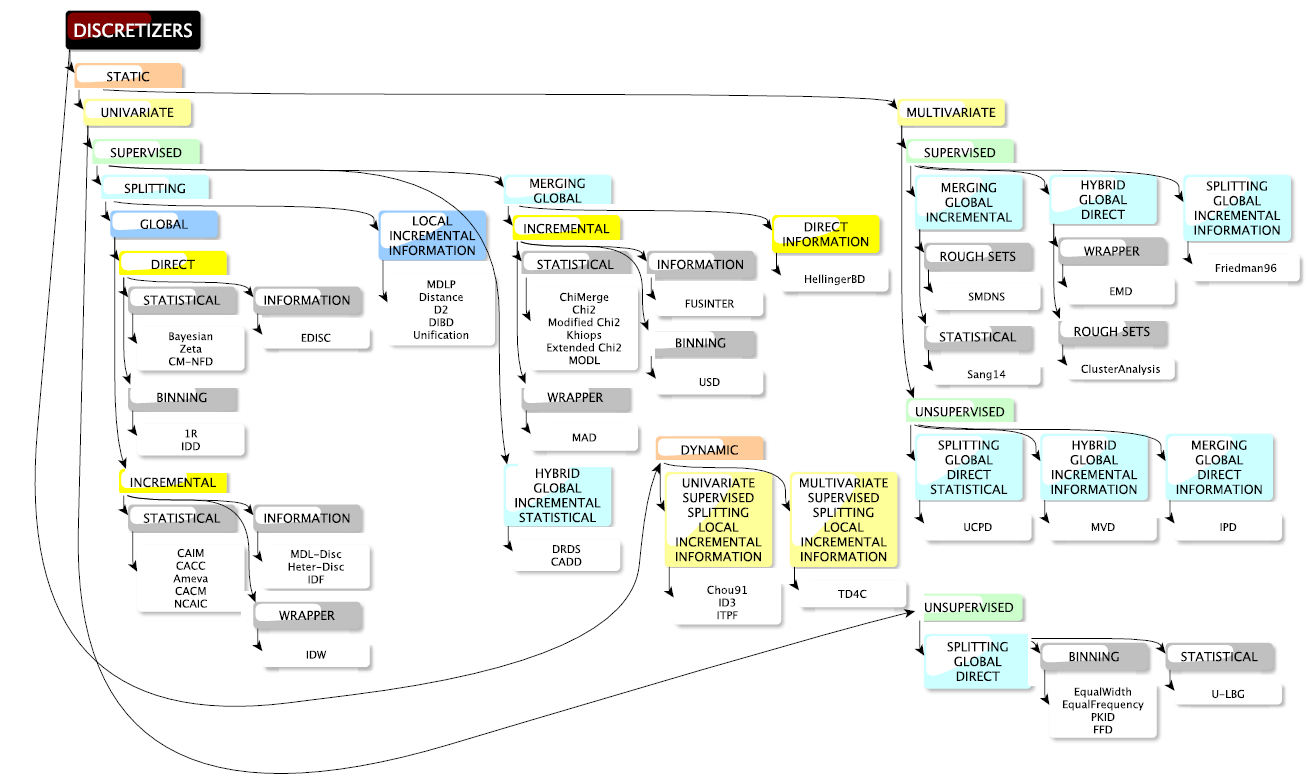
\includegraphics[scale=0.3]{figures/taxonomy.PNG}
\end{center}
\vspace*{-0.2cm}
These approaches (\cite{wrapper2}) maximize an ``intermediary'' criterion, \textit{e.g.}:
\vspace*{-0.1cm}
\begin{minipage}[c]{0.15\linewidth}
\begin{animateinline}[autoplay,loop]{2}%
{\color{orange}{\bf CACF}}%
\newframe \end{animateinline}
\end{minipage}
\begin{minipage}[c]{0.8\linewidth}
\[ \hat{\q}_j^{\chi^2} = \argmax_{\q_j} \chi^2(\q_j(\mathbf{x}_\text{f}), \mathbf{y}_\text{f}) \stackrel{?}{\approx} \q^\star_j, \]
\end{minipage}
\vspace*{-0.1cm}
and we {\bf hope} that it's aligned with our original goal s.t.:
%\vspace*{-0.1cm}

\begin{minipage}[c]{0.15\linewidth}
\begin{animateinline}[autoplay,loop]{2}%
{\color{orange}{\bf CACF}}%
\newframe \end{animateinline}
\end{minipage}
\begin{minipage}[c]{0.8\linewidth}
\[ \hat{\bm{\theta}}^{\chi^2} = \argmax_{\bm{\theta}} \ell(\bm{\theta} ; \mathbf{y}_\text{f}, {\hat{\q}^{\chi^2}}(\mathbf{x}_\text{f})) \stackrel{?}{\approx} \bm{\theta}^\star. \]
\end{minipage}

\end{frame}






\subsection{approximation}
\begin{frame}
\frametitle{\secname: \subsecname}

%%%%%%%%%
\note{
On a décidé de prendre une toute autre proche, toujours dans l'espoir d'apporter une formalisation et une résolution plus directe au problème original de sélection de modèle.

\bigskip

La première difficulté réside dans le fait que la quantification est un problème discret qu'on peut donc difficilement optimiser directement sans tester toutes les combinaisons

\bigskip

C'est pourquoi on relaxe le problème en paramétrant la quantification q par alpha, c'est-à-dire à utiliser des fonctions "douces", continues et dérivables de type softmax.

\bigskip

On peut l'interpréter comme la possibilité d'être dans plusieurs intervalles simultanément à des proportions différentes, ce qu'on peut simplement illustrer...


}
%%%%%%%%%



\begin{equation*}
    \q_{\ag_j}(\cdot)=\left(q_{\ag_{j,h}}(\cdot)\right)_{h=1}^{m_j} \text{ with } \begin{cases} \sum_{h=1}^{m_j}q_{\ag_{j,h}}(\cdot)=1, \\ 0 \leq q_{\ag_{j,h}}(\cdot) \leq 1, \end{cases}
\end{equation*}

\uncover<2->{

\textbf{For continuous features}, we set for $\bm{\alpha}_{j,h} = (\alpha^0_{j,h},\alpha^1_{j,h}) \in \mathbb{R}^2$
\[\s_{\ag_{j,h}}(\cdot) = \frac{\exp(\alpha^0_{j,h} + \alpha^1_{j,h}  \cdot)}{\sum_{g=1}^{m_j} \exp(\alpha^0_{j,g} + \alpha^1_{j,g}  \cdot)}.\]
}
\uncover<3->{
\textbf{For categorical features}, we set for $\bm{\alpha}_{j,h}=\left(\alpha_{j,h}(1),\ldots, \alpha_{j,h}(l_j)\right) \in \mathbb{R}^{l_j}$
\[\s_{\ag_{j,h}}(\cdot) = \frac{\exp\left(\alpha_{j,h}(\cdot)\right)}{\sum_{g=1}^{m_j} \exp\left(\alpha_{j,g}(\cdot)\right)}.\]
}

\end{frame}





\subsection{estimation MAP}
\begin{frame}
\frametitle{\secname : \subsecname}


%%%%%%%%%%
\note{

... avec 3 softmax cherchant à estimer 3 vraies quantifications dont les points de coupure sont en orange

\bigskip

Dans cet exemple, on a par exemple une proba de 80 pourcent d'être dans le premier intervalle, de 15 pourcent dans le second et de 5 pourcent dans le dernier.

\bigskip

A supposer qu'on puisse estimer les paramètres alpha chapeau donnés ici, on peut même "forcer" la quantification "douce" q alpha à redevenir une vraie quantification, c'est-à-dire des créneaux, en réalisant une estimation du maximum a posteriori : là où la première modalité est "majoritaire" donc > 33 pourcent dans cet exemple, on considère que c'est le premier intervalle. Ca nous permet de retrouver les points de coupure orange.

}
%%%%%%%%%%


\vspace*{-0.2cm}

\[ \hat{\s}_{j,h}(x_j) = 1 \text{ if } h = \argmax_{1 \leq h' \leq m_j} \s_{\hat{\ag}_{j,h'}}, 0 \text{ otherwise.} \]

\begin{tikzpicture}[scale=0.9]
\begin{axis}[
  no markers, domain=-1.5:2, samples=100,
  axis lines*=left,
  every axis y label/.style={at=(current axis.left of origin), anchor=north west},
  height=3cm, width=11cm,
  xtick=\empty, ytick=\empty,
  enlargelimits=false, clip=false,
  x label style={at={(axis description cs:0.5,0)},anchor=north},
  y label style={at={(axis description cs:-0.1,.5)},rotate=90,anchor=south},
  xlabel={$x_j$},
  ylabel={$\s_{\hat{\ag}_{j,1}}(x_j)$}
  ]
    
  \addplot [very thick,white] {gauss(-1.8,0.6)};
\addplot+[mark=none,ultra thick,orange] coordinates {(-0.7,0) (-0.7,0.6)};
\addplot+[mark=none,ultra thick,orange] coordinates {(1,0) (1,0.6)};
\node at (axis cs:-1.1,0.4) {$\hat{\s}_{j,1}(x_j)=1$};
\node at (axis cs:0,0.4) {$\hat{\s}_{j,1}(x_j)=0$};
\node at (axis cs:1.5,0.4) {$\hat{\s}_{j,1}(x_j)=0$};
\node at (axis cs:-0.7,-0.15) {$\hat{c}_{j,1}$};
\node at (axis cs:1,-0.15) {$\hat{c}_{j,2}$};

\end{axis}
\end{tikzpicture}

\begin{tikzpicture}[scale=0.9]
\begin{axis}[
  no markers, domain=-1.5:2, samples=100,
  axis lines*=left,
  every axis y label/.style={at=(current axis.left of origin), anchor=north west},
  height=3cm, width=11cm,
  xtick=\empty, ytick=\empty,
  enlargelimits=false, clip=false,
  x label style={at={(axis description cs:0.5,0)},anchor=north},
  y label style={at={(axis description cs:-0.1,.5)},rotate=90,anchor=south},
  xlabel={$x_j$},
  ylabel={$\s_{\hat{\ag}_{j,2}}(x_j)$}
  ]
    
  \addplot [very thick,white] {gauss(0,0.6)};
\addplot+[mark=none, ultra thick,orange] coordinates {(-0.7,0) (-0.7,0.6)};
\addplot+[mark=none, ultra thick,orange] coordinates {(1,0) (1,0.6)};
\node at (axis cs:-1.1,0.4) {$\hat{\s}_{j,2}(x_j)=0$};
\node at (axis cs:0,0.4) {$\hat{\s}_{j,2}(x_j)=1$};
\node at (axis cs:1.5,0.4) {$\hat{\s}_{j,2}(x_j)=0$};
\node at (axis cs:-0.7,-0.15) {$\hat{c}_{j,1}$};
\node at (axis cs:1,-0.15) {$\hat{c}_{j,2}$};

\end{axis}

\end{tikzpicture}

\begin{tikzpicture}[scale=0.9]
\begin{axis}[
  no markers, domain=-1.5:2, samples=100,
  axis lines*=left,
  every axis y label/.style={at=(current axis.left of origin), anchor=north west},
  height=3cm, width=11cm,
  xtick=\empty, ytick=\empty,
  enlargelimits=false, clip=false,
  x label style={at={(axis description cs:0.5,0)},anchor=north},
  y label style={at={(axis description cs:-0.1,.5)},rotate=90,anchor=south},
  xlabel={$x_j$},
  ylabel={$\s_{\hat{\ag}_{j,3}}(x_j)$}
  ]
    
  \addplot [very thick,white] {gauss(2,0.6)};

\addplot+[mark=none, ultra thick,orange] coordinates {(-0.7,0) (-0.7,0.6)};
\addplot+[mark=none, ultra thick,orange] coordinates {(1,0) (1,0.6)};

\node at (axis cs:-1.1,0.4) {$\hat{\s}_{j,3}(x_j)=0$};
\node at (axis cs:0,0.4) {$\hat{\s}_{j,3}(x_j)=0$};
\node at (axis cs:1.5,0.4) {$\hat{\s}_{j,3}(x_j)=1$};
\node at (axis cs:-0.7,-0.15) {$\hat{c}_{j,1}$};
\node at (axis cs:1,-0.15) {$\hat{c}_{j,2}$};

\end{axis}
\end{tikzpicture}


\end{frame}





\subsection{neural networks}

\begin{frame}
\frametitle{\secname: \subsecname}


%%%%%%%%%%
\note{
Pour estimer de bons paramètres alpha, on se plonge encore une fois dans le cadre de la vraisemblance...

\bigskip

... qu'on aimerait maximiser en $\theta$ et $\alpha$ ce qui nous conduirait, d'après les propriétés du maximum de vraisemblance, à retrouver au moins asymptotiquement le vrai mécanisme de génération des données, c-à-d la vraie quantification

\bigskip

sauf que on ne peut pas maximiser cette vraisemblance directement, donc on utilise également une heuristique : la descente de gradient.

}
%%%%%%%%%%



We wish to maximize the following likelihood:
\[ (\hat{\bm{\theta}}, \hat{\bm{\alpha}}) = \argmax_{\bm{\theta}, \bm{\alpha}} \ell(\bm{\theta}, \bm{\alpha} ; \bm{\mathbf{x}}_\f, \bm{\mathbf{y}}_\f) = \argmax_{\bm{\theta}, \bm{\alpha}} \sum_{i=1}^n \ln p_{\bm{\theta}}(y_i | \q_{\alpha}(\bm{x}_i)). \]

\medskip

{\bf If there is a true quantization} $\q^\star$, then $\bm{\alpha}^\star = \lim_{n \to \infty} \hat{\bm{\alpha}}$ is such that $\q_{\bm{\alpha}^\star} = \q^\star$.

\medskip

\uncover<2->{
{\bf If not}, $\hat{\q}$ is ``guaranteed'' to be a good candidate quantization.
}

\medskip

\uncover<3->{
{\bf Problem:} $\ell(\bm{\theta}, \bm{\alpha} ; \bm{\mathbf{x}}_\f, \bm{\mathbf{y}}_\f)$ cannot be directly maximized (it's not even convex).
}

\medskip

\uncover<4->{
{\bf Solution:} Resort to gradient descent (not guaranteed to converge to a global maximum!).
}

\end{frame}






\begin{frame}
\frametitle{\secname: \subsecname}

%%%%%%%%%%
\note{C'est là que la paramétrisation sous la forme de softmax prend son sens puisqu'on peut écrire le modèle comme un réseau de neurones très simple.

\bigskip

On peut donc s'appuyer sur les librairies logicielles standards de réseaux de neurones, qui marchent bien et très vite.
}
%%%%%%%%%%


Very simple neural network.

Very fast implementations available, \textit{e.g.}\ TensorFlow.

\textbf{No guarantee} of global optimum (but works well in practice).

\def\layersep{2.5cm}

\centering
\begin{tikzpicture}[shorten >=1pt,->,draw=black!50, node distance=\layersep]
    \tikzstyle{every pin edge}=[<-,shorten <=1pt]
    \tikzstyle{neuron}=[circle,fill=black!25,minimum size=17pt,inner sep=0pt]
    \tikzstyle{input neuron}=[neuron, fill=green!50];
    \tikzstyle{output neuron}=[neuron, fill=red!50];
    \tikzstyle{hidden neuron}=[neuron, fill=blue!50];
    \tikzstyle{annot} = [text width=4em, text centered]
    \tikzstyle{annotrectangle} = [text width=8em, text centered]


        \node[input neuron, pin=left:Continuous input \#1] (I-1) at (0,-1) {};
        
        \node[input neuron, pin=left:Level \#1] (I-2) at (0,-2) {};
        \node[input neuron, pin=left:Level \#2] (I-3) at (0,-3) {};
        \node[input neuron, pin=left:Level \#3] (I-4) at (0,-4) {};

    % Draw the hidden layer nodes
    \foreach \name / \y in {1,...,2}
        \path[yshift=0.5cm]
            node[hidden neuron] (H-\name) at (\layersep,-\y cm) {Soft};

    \foreach \name / \y in {3,...,4}
        \path[yshift=0.5cm]
            node[hidden neuron] (H-\name) at (\layersep,-\y cm) {Soft};

    % Draw the output layer node
    \node[output neuron,pin={[pin edge={->}]right:Output}, right of=H-2] (O) {$\sigma$};

    % Connect every node in the input layer with every node in the
    % hidden layer.
%    \foreach \source in {1,...,4}
        \foreach \dest in {1,2}
            \path (I-1) edge (H-\dest);

        \foreach \dest in {3,4}
            \path (I-2) edge (H-\dest);
        \foreach \dest in {3,4}
            \path (I-3) edge (H-\dest);
        \foreach \dest in {3,4}
            \path (I-4) edge (H-\dest);

        % \foreach \dest in {5,6}
        %     \path (I-3) edge (H-\dest);

    % Connect every node in the hidden layer with the output layer
    \foreach \source in {1,...,4}
        \path (H-\source) edge (O);

    % Annotate the layers
    \node[annot,above of=H-1, node distance=1cm] (hl) {Hidden layer};
    \node[annot,left of=hl] {Input layer};
    \node[annot,right of=hl] {Output layer};
    
    
    \draw [orange] (2,0) rectangle (3,-1.9);
    % \draw [red] (2,-2) rectangle (3,-4);
    
    \node[annotrectangle,right of=H-1, node distance=2.5cm] {Softmax outputs are $\q_{{\ag}_j}(x_j)$.}; 
    

\end{tikzpicture}

\end{frame}





\newlength\figureheight
\newlength\figurewidth
\setlength\figureheight{7cm}
\setlength\figurewidth{12cm}
 
\begin{frame}
\frametitle{\secname: \subsecname}

%%%%%%%%%%
\note{On peut donc regarder les estimations successives des paramètres alpha et les quantifications "douces" qui en résultent quand on simule une vraie discrétisation à 3 modalités avec 5 softmax (donc 5 modalités au maximum).

\bigskip

Les vrais points de coupure sont en pointillés (1/3 et 2/3).

\bigskip

Au départ, seuls 2 softmax s'activent et au fur et à mesure des itérations, on a bien 3 softmax qui ressemblent à des créneaux.
}
%%%%%%%%%%



\begin{figure}
\hspace*{-1cm}
%\begin{animateinline}[poster=first, controls, buttonfg=white]{3}
%\multiframe{200}{i=1+1}{\input{CODE_FIGURES/GLMDISC_NN/feature_0_iteration_\i.tex}}%
%\end{animateinline}
\end{figure}

\end{frame}





\subsection{model = quantization selection}

\begin{frame}
\frametitle{\secname : \subsecname}


%%%%%%%%%%
\note{
Ces pas de descente de gradient fournissent autant de quantifications candidates, a priori tournant en distribution autour du lieu du maximum de vraisemblance, que l'on peut passer à la moulinette du critère de sélection de modèle qu'on s'est donné au départ, BIC ici.

\medskip

Un élément important caché dans la présentation est le nombre de modalités que l'on cherche par variable quantifié, que l'on range dans le vecteur m et qui était en fait fixé par la structure du réseau de neurones : c'est-à-dire que sur l'exemple précédent, si on se done 5 softmax, on ne pourra avoir plus de 5 modalités à la fin.

\medskip

Il faudrait donc a priori boucler sur ce paramètre vectoriel discret, ce qui est bien moins combinatoire que le problème de départ mais quand même intractable.

\medskip

En pratique comme on l'a vu sur l'exemple, sur le support des observations de la variable prédictive, on a d'abord 2 puis 3 modalités seulement, ce qui était le vrai nombre de modalités, alors qu'on pouvait en avoir au maximum 5.

\medskip

Autrement dit, on peut se permettre de fixer cet hyperparamètre à un nombre maximum et laisser le critère de sélection de modèle opérer.

}
%%%%%%%%%%


\begin{block}{Quantization provider to original selection criterion}
We have drastically restricted the search space to \textit{iter} well-chosen candidates resulting from the the gradient descent steps.
\[ s^\star = \argmin_{s = 1, \ldots, \textit{iter}} \text{BIC}(\hat{\bth}_{\hat{\q}^{(s)}}) \]
\end{block}

\medskip

\uncover<2->{
We would still need to loop over candidates $\textcolor{yellow}{\bm{m}}$!
}

\medskip

\uncover<3->{
In practice if $\forall i, \; q_{\alpha_{j,h}}(x_j) \ll 1$, then level $h$ disappears while performing the $\argmax$.
}

\medskip

\uncover<4->{
Start with $\bm{m} = (m_{\text{max}})_1^d$ and ``wait'' \dots
}


\end{frame}








\subsection{results}

\begin{frame}

\frametitle{\secname: \subsecname}


%%%%%%%%%%
\note{
On peut vérifier la consistance empirique de l'approche proposée en simulant les mêmes données que sur l'exemple.

\bigskip

On s'aperçoit qu'on estime très bien les points de coupure et le vrai nombre de modalités.

\bigskip

On arrive même à faire de la sélection de variable puisqu'en ajoutant une variable $x_3$ qui n'apporte rien à la prédiction de $y$, on produit dans 88 cas sur 100 une seule modalité de quantification, c-à-dire que la variable sort du modèle.

}
%%%%%%%%%%



Simulated data

\medskip

\begin{table}[ht]
    \centering
    \caption{For different sample sizes $n$, (A) CI of $\hat{c}_{j,2}$ for $c_{j,2} = 2/3$. (B) CI of $\hat{m}$ for $m_1=3$. (C) CI of $\hat{m}_3$ for $m_3=1$.}
    \label{tab:estim_precision}
\begin{tabular}{llllll}
$n$ & (A) $\hat{c}_{j,2}$ & (B) & $\hat{m}_1$ & (C) & $\hat{m}_3$ \\
\hline
$1{,}000$ & $[0.656,0.666]$ & \myobar{1}{90}{9} & \mybar{60}{32}{8} \\
$10{,}000$ & $[0.666,0.666]$ & \myobar{0}{100}{0} & \mybar{88}{12}{0}
\end{tabular}
\end{table}

\end{frame}






\begin{frame}
\frametitle{\secname: \subsecname}


%%%%%%%%%%
\note{
Sur des données de benchmark du répertoire UCI avec des données mixtes, on se compare ensuite à la régression logistique linéaire, qui ne montre jamais la meilleure performance sur ces exemples, aux méthodes ad hoc de type Chi 2 pour les catégoriels et MDLP pour les continus.

\medskip

On a appelé l'approche présentée jusqu'à présent glmdisc-NN pour réseau de neurones, on avait également développé un autre algorithme d'optimisation basé sur l'algorithme EM et sur lequel on a bati la brique de recherche d'interactions

\medskip

Pour rappel, ce sont des paires de prédicteurs, quantifiés, dont on fait une sorte de produit. Ca revient à estimer un coefficient de régression logistique pour chaque combinaison des deux prédicteurs. La recherche se fait dans un espace encore beaucoup plus grand que l'espace de quantification seul mais permet potentiellement de réduire encore le biais de modèle en flexibilisant la régression logistique.

\medskip

Sauf pour le premier jeu de données, on obtient systématiquement les meilleurs résultats avec l'une des 2 techniques d'optimisation et éventuellement les interactions...

}
%%%%%%%%%%





Données UCI

\begin{table}
    \centering
        \caption{Gini indices (the greater the value, the better the performance) of our proposed quantization algorithm \textit{glmdisc} and two baselines.}
    \label{tab:banchmark_inter}
\resizebox{\textwidth}{!}{
\begin{tabular}{llllll}
Dataset & ALLR & \textit{ad hoc} methods & \makecell{Our proposal:\\ \textit{glmdisc}-NN} & \makecell{Our proposal:\\ \textit{glmdisc}-SEM} & \makecell{\textit{glmdisc}-SEM\\ w.\ interactions} \\
\hline
Adult & 81.4 (1.0) & \textcolor{green}{\textbf{85.3}} (0.9) & 80.4 (1.0) & 81.5 (1.0) & 81.5 (1.0 - no interaction) \\
Australian & 72.1 (10.4) & 84.1 (7.5) & 92.5 (4.5) & \textcolor{green}{\textbf{100}} (0) & \textcolor{green}{\textbf{100}} (0 - no interaction) \\
Bands & 48.3 (17.8) & 47.3 (17.6) & 58.5 (12.0) & \textcolor{green}{\textbf{58.7}} (12.0) & \textcolor{green}{\textbf{58.8}} (13.0) \\
Credit & 81.3 (9.6) & 88.7 (6.4) & \textcolor{green}{\textbf{92.0}} (4.7) & 87.7 (6.4) & 87.7 (6.4 - no interaction) \\
German & 52.0 (11.3) & 54.6 (11.2) & \textcolor{green}{\textbf{69.2}} (9.1) & 54.5 (10) & 56.5 (9.0) \\
Heart & 80.3 (12.1) & 78.7 (13.1) & \textcolor{green}{\textbf{86.3}} (10.6) & 82.2 (11.2) & 84.5 (10.8)
\end{tabular}
}
\end{table}

\end{frame}





\begin{frame}
\frametitle{\secname : \subsecname}


%%%%%%%%%%
\note{
Ce qu'on peut également vérifier sur d'autres types de données disponibles dans R où la régression logistique, éventuellement avec interactions est souvent utilisée, en l'occurence les applications médicales

\bigskip

Les interactions prennent tout leur sens et produisent les meilleurs résultats, sauf pour le jeu de données Pima où la régression logistique linéaire donne les meilleurs résultats

}
%%%%%%%%%%




Medicine data

\begin{table}[t]
\begin{center}
\caption{Gini indices of our proposed quantization algorithm \textit{glmdisc}-SEM and two baselines.}
\label{tab:banchmark_medicine}
\begin{adjustbox}{max width=0.99\textwidth}
\begin{tabular}{rrrrr}
 & Pima & Breast & Birthwt \\ 
  \hline
ALLR & {\textcolor{green}{\textbf{73.0}}} & 94.0 & 34.0 \\ 
ALLR LR w. interactions & 60.0 & 51.0 & 15.0 \\ 
glmdisc & 57.0 & 93.0 & 18.0 \\ 
glmdisc w. interactions & 62.0 & \textcolor{green}{\textbf{95.0}} & \textcolor{green}{{\textbf{54.0}}}\\ 
\end{tabular}
\end{adjustbox}
\end{center}
\end{table}


\end{frame}





\begin{frame}
\frametitle{\secname : \subsecname}

%%%%%%%%%%
\note{
On vérifie bien sûr que ça fonctionne sur les données CACF où on obtient aussi de très bons résultats, sauf qu'ils sont rarement significativement meilleurs.

\bigskip

Néanmoins, le gain principal de cette partie de thèse pour CACF se situe plutôt dans le gain de temps significatif du chargé d'études statistiques qui consacre un bon mois à la quantification pour la construction d'un score, ce qui est ici substitué par du temps machine.

\bigskip

De plus, on utilise la même dizaine de données depuis assez longtemps, donc a priori on est très proche de l'erreur de Bayes même avec des données quantifiées manuellement.
}
%%%%%%%%%%





CACF data

\begin{table}
    \centering
        \caption{Gini indices (the greater the value, the better the performance) of our proposed quantization algorithm \textit{glmdisc}, the two baselines and the current scorecard.}
    \label{tab:real_data_inter}
\resizebox{\textwidth}{!}{
\begin{tabular}{lllllll}
Portfolio & ALLR & \makecell{Current\\performance} & \makecell{\textit{ad hoc}\\methods} & \makecell{Our proposal:\\ \textit{glmdisc}-NN} & \makecell{Our proposal:\\ \textit{glmdisc}-SEM} & \makecell{\textit{glmdisc}-SEM\\ w.\ interactions} \\
\hline
Automobile & 59.3 (3.1) & 55.6 (3.4) & 59.3 (3.0) & 58.9 (2.6) & 57.8 (2.9) & \textcolor{green}{\bf{64.8}} (2.0) \\
Renovation & 52.3 (5.5) & 50.9 (5.6) & 54.0 (5.1) & \textcolor{green}{\bf{56.7}} (4.8) & 55.5 (5.2) & 55.5 (5.2) \\
Standard & 39.7 (3.3) & 37.1 (3.8) & 45.3 (3.1) & 43.8 (3.2) & 36.7 (3.7) & \textcolor{green}{\bf{47.2}} (2.8) \\
Revolving & 62.7 (2.8) & 58.5 (3.2) & 63.2 (2.8) & 62.3 (2.8) & 60.7 (2.8) & \textcolor{green}{\bf{67.2}} (2.5) \\
Mass retail & 52.8 (5.3) & 48.7 (6.0) & 61.4 (4.7) & \textcolor{green}{\bf{61.8}} (4.6) & 61.0 (4.7) & 60.3 (4.8) \\
Electronics & 52.9 (11.9) & 55.8 (10.8) & 56.3 (10.2)  & \textcolor{green}{\bf{72.6}} (7.4) & 62.0 (9.5) & 63.7 (9.0) \\
\end{tabular}
}
\end{table}


\end{frame}










\section{Segmentation: logistic regression trees}

\note{Ce qui apparaît sur le dernier tableau qu'on a vu, c'est que CACF dispose de pleins de segments de clientèle ou de portefeuilles sur lesquels il y a en fait des scores différents, alors que jusqu'à présent on s'est intéressé à un seul score.
}

{
\setbeamercolor{background canvas}{bg=white}

\begin{frame}
\frametitle{\secname}




%%%%%%%%%%
\note{Un score est spécifique à un segment de clientèle. La segmentation de la clientèle peut se schématiser comme une arbre de décision. Arbre classique : les noeuds sont déterministes en fonction du produit financé p.ex. ; les feuilles sont des régression logistiques : des scores.}
%%%%%%%%%%



\tikzstyle{level 1}=[level distance=2cm, sibling distance=10cm]
\tikzstyle{level 2}=[level distance=2cm, sibling distance=4.7cm]
\tikzstyle{level 3}=[level distance=2cm, sibling distance=3.8cm]

\begin{figure}
\centering

\resizebox{\linewidth}{!}{\begin{tikzpicture}
  [
    sibling distance        = 15em,
    level distance          = 5em,
    edge from parent/.style = {draw = black, -latex},
    every node/.style       = {font=\large},
    sloped
  ]
  \node [root] {\textcolor{black}{Clients}}
    child { node [dummy] {}
      child { node [dummy] {}
        child { node [env] {\textcolor{black}{$p_{\theta_1}(y|\bm{q}_{\{1\}}(\bm{x}_{\{1\}}))$}}
          edge from parent node [below] {\textcolor{black}{Renters}} }
        child { node [env] {\textcolor{black}{$p_{\theta_2}(y|\bm{q}_{\{2\}}(\bm{x}_{\{2\}}))$}}
          edge from parent node [above] {\textcolor{black}{Workers}} }
        child { node [env] {\textcolor{black}{$p_{\theta_3}(y|\bm{q}_{\{3\}}(\bm{x}_{\{3\}}))$}}
                edge from parent node [above] {\textcolor{black}{Others}} }
        edge from parent node [above] {\textcolor{black}{Revolving}} }
      child { node [env] {\textcolor{black}{$p_{\theta_4}(y|\bm{q}_{\{4\}}(\bm{x}_{\{4\}}))$}}
              edge from parent node [above, align=center]
                {\textcolor{black}{Standard}} }
              edge from parent node [above] {\textcolor{black}{Appliances}} }
    child { node [dummy] {}
      child { node [dummy] {}
        child { node [env] {\textcolor{black}{$p_{\theta_5}(y|\bm{q}_{\{5\}}(\bm{x}_{\{5\}}))$}}
          edge from parent node [above] {\textcolor{black}{Leasing}} }
        child { node [env] {\textcolor{black}{$p_{\theta_6}(y|\bm{q}_{\{6\}}(\bm{x}_{\{6\}}))$}}
                edge from parent node [above] {\textcolor{black}{Standard}} }
        edge from parent node [above] {\textcolor{black}{Fiat}} }
      child { node [env] {\textcolor{black}{$p_{\theta_7}(y|\bm{q}_{\{7\}}(\bm{x}_{\{7\}}))$}}
              edge from parent node [above, align=center]
                {\textcolor{black}{Kawasaki}} }
              edge from parent node [above] {\textcolor{black}{Cars}} };
\end{tikzpicture}}
\caption{\textcolor{black}{Scorecards tree structure in acceptance system.} }
\label{fig:arbre}
\end{figure}

\end{frame}


}

\setbeamercolor{normal text}{fg=white}
\usebeamercolor[fg]{normal text}


\begin{frame}
\frametitle{\secname}


%%%%%%%%%%%
\note{Au moment d'un appel d'offre et pour la conquête d'un nouveau partenaire.

\bigskip

Performance et variables utilisés similaires.

\bigskip

Au moment de la création d'un score comme sur la slide d'introduction du contexte industriel en début de présentation.

\bigskip

On se propose de se replonger dans un cadre académique en simulant des données qui vont faire échouer la pratique industrielle de l'ACM}
%%%%%%%%%%%


Current procedure(s):
\begin{itemize}
\item<2-> Promise a new partner their own score to maximize acceptance;
\item<3-> Merge existing ``close'' branches that show similar performance;
\item<4-> \begin{minipage}[c]{0.1\linewidth}
\only<4->{\begin{animateinline}[autoplay,loop]{2}%
{\color{orange}{\bf CACF}}%
\newframe \end{animateinline}}
\end{minipage}
\begin{minipage}[c]{0.85\linewidth}
Try basic ``clustering'' techniques, \textit{e.g.}\ MCA.
\end{minipage}
\end{itemize}

\bigskip

\uncover<5->{
Problem(s):
\begin{itemize}
\item<6-> This structure is not the result of optimization and is probably suboptimal (by how much?);
\item<7-> There are situations in which it severely fails.
\end{itemize}
}

\end{frame}




\begin{frame}
\frametitle{\secname}

%%%%%%%%%%%%%%%%%%%
\note{On simule trois clusters apparents : les classes populaires, moyennes et aisées.

\bigskip

Leur performance de remboursement est néanmoins déterminé dans tous les cas par leur taux d'endettement.

\bigskip

Le vrai modèle est donc constitué d'une seule régression logistique là où une approche de type ACM va choisir de réaliser trois régressions.}
%%%%%%%%%%%%%%%%%%%


\hspace*{-2cm}\resizebox{1.2\textwidth}{!}{
\begin{tikzpicture}[
    declare function={a(\x)=0.75*\x-2;},
    declare function={b(\x)=0.75*\x-1;}
]


\begin{axis}[xtick=\empty, ytick=\empty, xlabel={Revenus}, ylabel={Endettement}]
\myGlobalTransformation{0}{0};

% pauvres
\addplot [green, only marks, mark=*, samples=300, mark size=0.75,domain=-3:1]{rand+x};
\addplot [red, only marks, mark=*, samples=300, mark size=0.75,domain=-3:1]{rand+x+2.5};

%moyens
\addplot [green, only marks, mark=*, samples=300, mark size=0.75,domain=2:6]{rand+x};
\addplot [red, only marks, mark=*, samples=300, mark size=0.75,domain=2:6]{rand+x+2.5};

%riches
\addplot [green, only marks, mark=*, samples=300, mark size=0.75,domain=7:11]{rand+x};
\addplot [red, only marks, mark=*, samples=300, mark size=0.75,domain=7:11]{rand+x+2.5};

%frontière
\addplot [white, very thick, domain=-3:11] {x+1.25};
\end{axis}


\end{tikzpicture}
}

\end{frame}







\begin{frame}
\frametitle{\secname}


%%%%%%%%%%%%%%%%
\note{On simule trois régressions différentes déterminées par une variable catégorielle, par exemple la catégorie socio-professionnelle.

\bigskip

Une approche de type ACM, même en connaissant la variable catégorielle, ne pourra trouver qu'un seul cluster puisqu'on ne fournit pas la variable cible, et produira donc de très mauvais résultats prédictifs que l'on vérifiera à la fin de cette partie.}
%%%%%%%%%%%%%%%%


\begin{tikzpicture}


\begin{axis}[xtick=\empty, ytick=\empty, xlabel={Revenus}, ylabel={Endettement},domain=-3:1, enlargelimits=false,ymin=-3,ymax=6]
\myGlobalTransformationbis{0}{0};

% techniciens
\addplot [green, only marks, mark=*, samples=300, mark size=0.75,domain=-3:1]{rand};
\addplot [green, only marks, mark=*, samples=300, mark size=0.75,domain=-3:1]{rand-2};
\addplot [green, only marks, mark=*, samples=300, mark size=0.75,domain=-3:1]{rand-4};
\addplot [red, only marks, mark=*, samples=300, mark size=0.75,domain=-3:1]{rand+2.5};
\addplot [red, only marks, mark=*, samples=300, mark size=0.75,domain=-3:1]{rand+4.5};
\addplot [red, only marks, mark=*, samples=300, mark size=0.75,domain=-3:1]{rand+6.5};

%frontière
\addplot [white, very thick, domain=-3:1] {1.25};
\end{axis}





\begin{axis}[xtick=\empty, ytick=\empty, xlabel={Revenus}, ylabel={Endettement},domain=-3:1, enlargelimits=false,ymin=-3,ymax=6]
\myGlobalTransformationbis{0}{3};

% cadres
\addplot [green, only marks, mark=*, samples=300, mark size=0.75,domain=-3:1]{rand-x};
\addplot [green, only marks, mark=*, samples=300, mark size=0.75,domain=-3:1]{rand-x-2};
\addplot [green, only marks, mark=*, samples=300, mark size=0.75,domain=-3:1]{rand-x-4};
\addplot [red, only marks, mark=*, samples=300, mark size=0.75,domain=-3:1]{rand-x+2.5};
\addplot [red, only marks, mark=*, samples=300, mark size=0.75,domain=-3:1]{rand-x+4.5};
\addplot [red, only marks, mark=*, samples=300, mark size=0.75,domain=-3:1]{rand-x+6.5};

%frontière
\addplot [white, very thick, domain=-3:1] {-x+1.25};
\end{axis}



\begin{axis}[xtick=\empty, ytick=\empty, xlabel={Revenus}, ylabel={Endettement},domain=-3:1, enlargelimits=false,ymin=-3,ymax=6]
\myGlobalTransformationbis{0}{6};

% libérales
\addplot [green, only marks, mark=*, samples=300, mark size=0.75,domain=-3:1]{rand+x};
\addplot [green, only marks, mark=*, samples=300, mark size=0.75,domain=-3:1]{rand+x-2};
\addplot [green, only marks, mark=*, samples=300, mark size=0.75,domain=-3:1]{rand+x-4};
\addplot [red, only marks, mark=*, samples=300, mark size=0.75,domain=-3:1]{rand+x+2.5};
\addplot [red, only marks, mark=*, samples=300, mark size=0.75,domain=-3:1]{rand+x+4.5};
\addplot [red, only marks, mark=*, samples=300, mark size=0.75,domain=-3:1]{rand+x+6.5};
\addplot [red, only marks, mark=*, samples=300, mark size=0.75,domain=-3:1]{rand+x+8.5};

%frontière
\addplot [white, very thick, domain=-3:1] {x+1.25};
\end{axis}



\end{tikzpicture}

\end{frame}







\subsection{notations}

\begin{frame}
\frametitle{\secname: \subsecname}

%%%%%%%%%%%%%%%%%%%%%%%%%%
\note{On introduit quelques notations spécifiques à la segmentation. Comme pour les problèmes précédents, on suppose l'existence d'une vraie segmentation, c'est-à-dire de $K^\star$ segments, d'une affectation de chaque client $c^\star$, et de régressions logistiques pour chaque segment $\bm{\theta}^{\star, c^\star}$.

\bigskip

On aimerait utiliser les outils standards de sélection de modèle, comme le critère BIC utilisé jusqu'à présent, sauf que l'espace des segmentations possibles est à nouveau un problème discret intractable.

\bigskip

Sans surprise, on va à nouveau relaxer ce problème et proposer un algorithme itératif générant quelques propositions pertinentes de segmentations.}
%%%%%%%%%%%%%%%%%%%%%%%%%%

%\setbeamercolor{normal text}{fg=white}
%\usebeamercolor[fg]{normal text}

$K$ segments.

\medskip

\uncover<2->{
$c \in \{1, \dots, K\}$: latent feature of the client's segment.
}

\medskip

\uncover<2->{
$\mathbf{c} = (c_1, \dots, c_n)$: segment for all $n$ clients.
}


\medskip

\uncover<3->{
We suppose there is a true segmentation $K^\star, c^\star$ and logistic regressions $\bm{\theta}^{\star, c^\star}$ at its leaves.
}

\medskip

\uncover<4->{
If we could evaluate all segmentations, the best one could be selected by

\begin{minipage}[c]{0.15\linewidth}
\only<4->{\begin{animateinline}[autoplay,loop]{2}%
{\color{orange}{\bf Statistician}}%
\newframe \end{animateinline}}
\end{minipage}
\begin{minipage}[c]{0.8\linewidth}
\vspace*{-0.5cm}
\[ \hspace*{0.6cm} (\hat{K}, \hat{\mathbf{c}}) = \argmin_{K,\mathbf{c}} \sum_{c=1}^K \text{BIC}(\hat{\bm{\theta}}^{c} ; \{(\bm{x}_i,y_i) | c_{i} = c, 1 \leq i \leq n\}),\]
\end{minipage}
where $\hat{\bm{\theta}}^c$ is the MLE of the logistic regression of segment $c$.
}

\end{frame}








\subsection{model proposal}

\begin{frame}
\frametitle{\secname: \subsecname}

%%%%%%%%%%%%%%%%%%%%%%%%%%%%%%
\note{
Comme pour la quantification où l'on pouvait être dans plusieurs modalités à la fois dans des proportions différentes, on autorise ici les clients à être dans plusieurs segments à la fois, ce qui revient à considérer un modèle de mélange régression logistique, prédisant le remboursement du client sachant ses prédicteurs et son segment d'appartenance et arbre de décision, prédisant l'appartenance à un segment donné.

D'un point de vue académique, on flexibilise la régression logistique par l'apport d'un modèle d'arbre non paramétrique tout en répondant à la contrainte industrielle d'interprétabilité.

Ici encore, on met en oeuvre un algorithme de type EM qui va tirer le segment d'appartenance de chaque client selon la probabilité donné par le mélange.

Une fois que l'on connait le segment d'appartenance, on peut estimer classiquement les paramètres de régression logistique de chaque segment et mettre à jour également le modèle d'arbre qui donne les segments.

Comme pour la quantification, cette procédure est répétée un nombre de fois raisonnable et donné par l'utilisateur et il ne reste qu'à passer ces segmentations dans la moulinette du critère de sélection de modèle choisi, par exemple BIC.}
%%%%%%%%%%%%%%%%%%%%%%%%%%%%%%





Similarly to the quantization proposal: ability to be in several segments at a time.

\medskip

\uncover<2->{
\[ p(y| \bm{x}) = \sum_{c=1}^K p_{\bm{\theta}}(y | \bm{x}; c) p_{\beta}(c | \bm{x}).\]
}

\medskip

\uncover<3->{
\[ c_i^{(s+1)} \sim p_{\bm{\theta}^{\cdot(s)}}(y_i | \bm{x}_i; \cdot) p_{\beta^{(s)}}(\cdot | \bm{x}_i). \]
}

\medskip

\uncover<4->{
\[ \bm{\theta}^{c(s+1)} = \argmax_{\bm{\theta}^c} \sum_{i=1}^n \mathds{1}_{c}(c_i^{s+1)}) \ln p_{\bm{\theta}^c}(y_i | \bm{x}_i ; c_i). \]
}

\medskip

\uncover<5->{
\[ \beta^{(s+1)} = \text{C4.5}(\mathbf{c}^{(s+1)}, \mathbf{x}) .\]
}

\end{frame}










\subsection{some results}

\begin{frame}
\frametitle{\secname: \subsecname}


%%%%%%%%%%%%%%%%%%%%%%%
\note{

Sur le premier jeu de données simulés présentés précédemment, le vrai modèle est une seule régression logistique qui est bien retrouvée par l'approche proposée à partir de 5 segments de départ. La méthode type ACM fait 3 régressions logistiques, toutes vraies également, mais qui utilisent moins de données et sont donc soumises à plus de variance, d'où le Gini plus faible.

Parmi deux autres approches d'arbres de régressions logistiques trouvés dans la littérature, LMT a également retrouvé un seul segment.

Pour le deuxième jeu de données, une seule régression logistique est trouvée par l'approche ACM puisqu'il n'y a pas de cluster apparent, d'où une performance faible. L'approche proposée retrouve bien les 3 segments. Pour les deux méthodes de la littérature, c'est cette fois MOB qui a bien retrouvé les 3 segments.

En conclusion, on a proposé une méthode qui permet de résoudre le problème académique posé au départ sur des données simulées ; il reste à l'appliquer sur des jeux de données réelles, où elle semble prometteuse mais d'autres problèmes restent à résoudre (notamment le temps de calcul avec des prédicteurs catégoriels).}
%%%%%%%%%%%%%%%%%%%%%%%%





\begin{table}[t]
\centering
\begin{tabular}{ll|lllll}
 & Oracle = ALLR & \textit{glmtree}-SEM & FAMD & LMT & MOB \\
\hline
Gini & 69.7 & \textcolor{green}{\textbf{69.7}} & 65.3 & \textcolor{green}{\textbf{69.7}} & 64.8 \\
\end{tabular}
\end{table}

\bigskip

\begin{table}[t]
\centering
\begin{tabular}{ll|llllll}
 & Oracle & ALLR & \textit{glmtree}-SEM & FAMD & LMT & MOB \\
\hline
Gini & 69.7 & 25.8 & \textcolor{green}{\textbf{69.7}} & 17.7 & 65.8 & \textcolor{green}{\textbf{69.7}} \\
\end{tabular}
\end{table}

\end{frame}













\section{Conclusion and future work}

\subsection{Conclusion}

\begin{frame}
\frametitle{\subsecname}


%%%%%%%%%%%%%%
\note{
En conclusion, cette thèse a permis de traiter trois problèmes inhérents au Credit Scoring:

\medskip

La réintégration des refusés, que l'on a reformulé comme un problème à variables manquantes, dont on a réinterprété certaines méthodes ad hoc. On ne regroupe aucune de ces méthodes, néanmoins elles sont implémentées dans un package R.

\medskip

Une sorte d'apprentissage de représentation sous contrainte des prédicteurs : la discrétisation ou le regroupement de modalités, la recherche d'interactions. On a replongé ce problème comme une sélection de modèle dans un très grand espace discret. On a proposé de relaxer ce problème, le rendre plus facile, et un mécanisme d'exploration intelligent de ce grand espace. On obtient de bonnes performances, et surtout un gain de temps significatif pour le statisticien. La méthode est implémentée dans un package R et Python.

\medskip

Enfin, la segmentation prédictive, c'est-à-dire les arbres de régression logistique où on a eu une approche similaire au problème de quantification, qui donne de très bons résultats sur les données simulées.
}
%%%%%%%%%%%%%%




This PhD tackled three main issues of ``traditional'' Credit Scoring:
\begin{enumerate}
\item Reject inference: impact of tossing away not-financed clients,

\medskip

\only<2>{Conclusion: sound problem reformulation, no method recommended, \lstinline{scoringTools} \textsc{R} package.}
\item<3-> ``Constrained'' representation learning: discretization, grouping, interaction screening,

\medskip

\only<4>{Conclusion: better performance, less time-consuming, some guarantees, \lstinline{glmdisc} \textsc{R} and Python packages.}
\item<5-> Predictive segmentation: logistic regression trees,

\medskip

\only<6>{Conclusion: first experiments on simulated and real data are encouraging, \lstinline{glmtree} \textsc{R} package.}
\end{enumerate}

\end{frame}




\subsection{Future work}

\begin{frame}
\frametitle{\subsecname}



%%%%%%%%%%%%%%
\note{
La poursuite des travaux de segmentation, en particulier sur des données réelles (même s'il y a déjà des premiers résultats), qui nécessiterait d'y inclure la quantification, la sélection de variables et éventuellement la recherche d'interactions, ce qui est un problème très combinatoire.

\medskip

Tous ces travaux concernent les pré-traitements des variables prédictives $x$, mais on pourrait s'intéresser à la définition de la variable cible, 2 mensualités impayées en un an, alors que l'objectif de l'institut financier est plutôt le profit.

\medskip

Enfin, à prédicteurs traditionnels fixes, toutes les ``optimisations'' dont on a parlé jusqu'à présent permettent essentiellement de gagner un temps significatif avec une augmentation faible à modérée de performance. Un vrai gain de performance éventuel viendrait sans doute avec la collecte et le traitement rigoureux de plus grandes quantités de données, en particulier les données non structurées et souvent très fines comme les données de cookies, de logs, de parcours de visite sur les sites internet, etc. ce qui est sans doute l'espoir majeur du Credit Scoring à moyen terme, et pourrait par exemple justifier une autre thèse CIFRE...
}
%%%%%%%%%%%%%%



There remains a lot of open questions:
\begin{enumerate}
\item Predictive segmentation: logistic regression trees,

\medskip

\only<2>{Perspective: allow for quantization / interaction screening and feature selection at each iteration.}
\item<3-> Credit Scoring for profit: swap ``$p($2 unpaid instalments$)$'' for $p($profit$>0)$ or $\mathbb{E}[\text{profit}]$,

\medskip

\only<4>{Perspective: experiment observation-wise misclassification costs.}
\item<5-> Representation learning for fine-grained unstructured data,

\medskip

\only<6>{Perspective: provide statistically sound methods to aggregate ``behavioural'' data, \textit{e.g.}\ web visitation patterns.}
\end{enumerate}

\end{frame}







\begin{frame}


%%%%%%%%%%%%%%
\note{... mais pour ma part j'en ai terminé ! Merci pour votre attention.}
%%%%%%%%%%%%%%

\Huge

Thanks!

\end{frame}






\begin{frame}[allowframebreaks]
\frametitle{References}
\begin{scriptsize}
\printbibliography
\end{scriptsize}
\end{frame}




\appendix


\section{Bivariate interactions}

\subsection{notations}

\begin{frame}
\frametitle{\secname: \subsecname}

Upper triangular matrix with $\delta_{k,\ell} = 1 $ if $k < \ell$ and features $k$ and $\ell$ ``interact'' in the logistic regression.
\[ \text{logit}(p_{\bm{\theta}}(1|\q(\bm{x}))) = \theta_0 + \sum_{j=1}^{d} \theta_j^{\q_j(x_j)} + \sum_{1\leq k < \ell \leq d} \delta_{k,\ell} \theta_{k,\ell}^{\q_k(x_k) f_{\ell}(x_{\ell})} \]
\uncover<2->{
Imagine for now that the discretization $\q(\bm{x})$ is fixed. The criterion becomes:
\begin{align*}
(\bm{\theta}^\star,\bm{\delta}^\star) & = \argmax_{\bm{\theta},\textcolor{yellow}{\bm{\delta} \in \{0,1\}^\frac{d(d-1)}{2}}} \sum_{i=1}^n \ln p_{\bm{\theta}}(y_i|\q(\bm{x}_i),\bm{\delta}) - \text{penalty}(n;\bm{\theta}) 
\end{align*}
}
\uncover<3->{
Analogous to previous problem: $2^{\frac{d(d-1)}{2}}$ models.
}


\end{frame}




\subsection{model proposal}
\begin{frame}
\frametitle{\secname: \subsecname}

$\delta$ is latent and hard to optimize over: use a stochastic algorithm!

\bigskip

\uncover<2->{
Strategy used here: Metropolis-Hastings sampling algorithm.

{\bf Idea:} propose well-chosen interactions and accept / reject them based on the BIC criterion of the resulting logistic regression.
}

\only<3>{
\begin{align*}
p(y|\bqk ) & = \sum_{\bm{\delta} \in \{0,1\}^\frac{d(d-1)}{2}} p(y | \bqk, \bm{\delta}) p(\bm{\delta}) \\
p(\bm{\delta} | \bqk,y) & \propto \exp(-\text{BIC}[\bm{\delta}]/2) p(\bm{\delta})
\end{align*}
}
\uncover<4->{
\begin{align*}
p(y| \bqk ) & = \sum_{\bm{\delta} \in \{0,1\}^\frac{d(d-1)}{2}} p(y | \bqk, \bm{\delta}) p(\bm{\delta}) \\
p(\bm{\delta} | \bqk,y) & \propto \exp(-\text{BIC}[\bm{\delta}]/2) \textcolor{yellow}{\cancel{p(\bm{\delta})}} \hspace{1cm} p(\delta_{p,q}) = \frac{1}{2}
\end{align*}
}
\uncover<5->{
Which transition proposal $\tr: ({\{0,1\}}^{\frac{d(d-1)}{2}},{\{0,1\}}^{\frac{d(d-1)}{2}}) \mapsto [0 ; 1]$?
}

\end{frame}



\begin{frame}
\frametitle{\secname: \subsecname}

$2^{d(d-1)}$ probabilities to calculate\dots

\bigskip

\uncover<2->{
\textbf{We restrict changes to only one entry $\delta_{k,\ell}$.}
}

\bigskip

\uncover<3->{
\textbf{Proposal:} gain/loss in BIC between \textcolor{yellow}{bivariate} models \textcolor{yellow}{with} / \textcolor{yellow}{without} the interaction.
}

\bigskip

\uncover<4->{
If the interaction between two features is meaningful when only these two features are considered, there is a good chance that it will be in the full multivariate model.
}

\bigskip

\uncover<5->{
\textbf{Trick:} alternate one discretization  / grouping step and one ``interaction'' step.
}

\end{frame}







\section{SEM-Gibbs quantization}

\begin{frame}
\frametitle{\secname}

Originally (and as implemented in the \textsc{R} package glmdisc), the optimization was a bit different:
\begin{itemize}
\item<2-> $\q$ is considered a latent (unobserved) feature;
\item<3-> A classical EM algorithm is intractable since it requires an Expectation step over all possible quantizations;
\item<4-> Solution: random draw $\approx$ Bayesian statistics;
\end{itemize}

\end{frame}


\begin{frame}
\frametitle{\subsecname: estimation}

``Classical'' estimation strategy with latent variables: EM algorithm.

\bigskip

\uncover<2->{
There would still be a sum over $\bm{\mathcal{Q}}_{\bm{m}}$: $p(y|\bm{x},\bm{\theta},\bm{\alpha}) = \sum_{\q \in \bm{\mathcal{Q}}_{\bm{m}}} p_{\bm{\theta}}(y|\q) \prod_{j=1}^d p_{\bm{\alpha}_j}(\q_j|x_j)$
}

\bigskip

\uncover<3->{
Use a Stochastic-EM! Draw $\q$ knowing that:
}
\medskip
\uncover<4->{
\[p(\q|\bm{x},y) = \underbrace{\dfrac{p_{\bm{\theta}}(y|\q) \prod_{j=1}^d p_{\bm{\alpha_j}}(\q_j|x_j)}{\sum_{\bm{q} \in \bm{\mathcal{Q}}_{\bm{m}}} p_{\bm{\theta}}(y|\q) \prod_{j=1}^d p_{\bm{\alpha}_j}(\q_j|x_j)}}_{\text{still difficult to calculate}}\]
}
\medskip
\uncover<5->{
Gibbs-sampling step:
\[p(\q_j|\bm{x},y,\q_{\{-j\}}) \propto p_{\bm{\theta}}(y|\q) p_{\bm{\alpha_j}}(\q_j|x_j)\]
}


\end{frame}




\begin{frame}
\frametitle{\secname: algorithm}

\tiny


\textbf{Initialization}


\medskip

$\left( \begin{array}{ccc}
x_{1,1} & \cdots & x_{1,d}  \\
 \vdots & \vdots & \vdots \\
 x_{n,1} & \cdots & x_{n,d} \end{array} \right)
\begin{array}{c}
\text{at random} \\
\Rightarrow \end{array}
\left( \begin{array}{ccc}
\q_{1,1} & \cdots & \q_{1,d}  \\
 \vdots & \vdots & \vdots \\
 \q_{n,1} & \cdots & \q_{n,d} \end{array} \right)$

\medskip

\textbf{Loop}

\medskip

$\left( \begin{array}{c}
y_1 \\
\vdots \\
y_n \end{array} \right)
\begin{array}{c}
\text{logistic} \\
\text{regression} \\
\Rightarrow \end{array}
\left( \begin{array}{ccc}
\q_{1,1} & \cdots & \q_{1,d}  \\
 \vdots & \vdots & \vdots \\
 \q_{n,1} & \cdots & \q_{n,d} \end{array} \right)
\begin{array}{c}
\text{polytomous} \\
\text{regression} \\
\Rightarrow \end{array}
\left( \begin{array}{ccc}
x_{1,1} & \cdots & x_{1,d}  \\
 \vdots & \vdots & \vdots \\
 x_{n,1} & \cdots & x_{n,d} \end{array} \right)
$

\medskip

\textbf{Updating $\q$}

\medskip

$\left( \begin{array}{c}
p(y_1,\q_{1,j}=k|\bm{x}_i)  \\
\vdots \\
p(y_n,\q_{n,j}=k|\bm{x}_i) \end{array} \right)
\begin{array}{c}
\text{random} \\
\text{sampling} \\
\Rightarrow \end{array}
\left( \begin{array}{ccc}
\q_{1,j}  \\
 \vdots \\
 \q_{n,j} \end{array} \right)$

\medskip

\textbf{Calculating $\q^{\text{MAP}}$}

\medskip

$\left( \begin{array}{c}
\q^{\text{MAP},1,j}  \\
\vdots \\
\q^{\text{MAP},n,j} \end{array} \right)
\begin{array}{c}
\text{MAP} \\
\text{estimate} \\
= \end{array}
\left( \begin{array}{ccc}
\argmax_{\q_j} p_{\bm{\alpha_j}}(\q_j | x_{1,j})  \\
 \vdots \\
\argmax_{\q_j} p_{\bm{\alpha_j}}(\q_j | x_{n,j}) \end{array} \right)$
 
 
\normalsize

\end{frame}






\begin{frame}
\frametitle{\secname : simulations}

\begin{figure}
%\begin{animateinline}[poster=first, controls, palindrome, buttonfg=white]{5}
%\multiframe{200}{i=1+1}{\input{CODE_FIGURES/GLMDISC_SEM/sem_feature_1_iter_\i.tex}}%
%\end{animateinline}
\end{figure}

\end{frame}


\end{document}


